    \documentclass[
		11pt,
		a4paper,
		titlepage=firstiscover,
	]{scrreprt}
	%----------------------------------------
% Basic Packages
%----------------------------------------
\usepackage[utf8]{inputenc}

\usepackage{pifont}
\usepackage{leftidx}

\usepackage[main=english, ]{babel}
\usepackage[x11names]{xcolor}
\usepackage{pdfpages}


\usepackage{pst-grad} % For gradients
\usepackage{pst-plot} % For axes


\usepackage[T1]{fontenc}
\usepackage{fancyhdr}



\usepackage[
bookmarksnumbered=true,
hidelinks,
bookmarksopen =true,
bookmarksdepth=2
]
{hyperref}

% widow/orphan 
\clubpenalty = 10000  
\widowpenalty = 10000 \displaywidowpenalty = 10000  


%%%----------------------------------------
% Drawings
%%%----------------------------------------	
\usepackage{tikz}	% for drawings

\usepackage{pgf}


\usepackage{pgfplots}
\pgfplotsset{compat=1.13}
 \usepgfplotslibrary{patchplots}
\tikzstyle{every pin}=[%fill=white,
					   %draw=black,
					   pin edge = black,
					   font=\footnotesize]
\pgfplotsset{every  tick/.style={black}}

\usepackage{pgffor} 
	\usetikzlibrary{arrows.meta}% Pfeile in TikZ
	\usetikzlibrary{positioning}% Pfeile in TikZ
	\usetikzlibrary{bending}% Pfeile in TikZ
	\usetikzlibrary{scopes} %for TikZ Scopes
	\usetikzlibrary{patterns} % fill patterns 
	\usetikzlibrary{fadings} % fading effects
	\usetikzlibrary{decorations.pathmorphing} %Freihandlinien 
	\usetikzlibrary{calc} %Vektorrechnung
	\usetikzlibrary{datavisualization} %Data Visualization
	\usetikzlibrary{datavisualization.formats.functions} %Function evaluation within Visualizations
	\usetikzlibrary{intersections} %calc intersections of paths	
	\usetikzlibrary{plotmarks}

	
% Box plots
\pgfplotsset{
    box plot/.style={
        /pgfplots/.cd,
        black,
        only marks,
        mark=-,
        mark size=\pgfkeysvalueof{/pgfplots/box plot width},
        /pgfplots/error bars/y dir=plus,
        /pgfplots/error bars/y explicit,
        /pgfplots/table/x index=\pgfkeysvalueof{/pgfplots/box plot x index},
    },
    box plot box/.style={
        /pgfplots/error bars/draw error bar/.code 2 args={%
            \draw  ##1 -- ++(\pgfkeysvalueof{/pgfplots/box plot width},0pt) |- ##2 -- ++(-\pgfkeysvalueof{/pgfplots/box plot width},0pt) |- ##1 -- cycle;
        },
        /pgfplots/table/.cd,
        y index=\pgfkeysvalueof{/pgfplots/box plot box top index},
        y error expr={
            \thisrowno{\pgfkeysvalueof{/pgfplots/box plot box bottom index}}
            - \thisrowno{\pgfkeysvalueof{/pgfplots/box plot box top index}}
        },
        /pgfplots/box plot
    },
    box plot top whisker/.style={
        /pgfplots/error bars/draw error bar/.code 2 args={%
            \pgfkeysgetvalue{/pgfplots/error bars/error mark}%
            {\pgfplotserrorbarsmark}%
            \pgfkeysgetvalue{/pgfplots/error bars/error mark options}%
            {\pgfplotserrorbarsmarkopts}%
            \path ##1 -- ##2;
        },
        /pgfplots/table/.cd,
        y index=\pgfkeysvalueof{/pgfplots/box plot whisker top index},
        y error expr={
            \thisrowno{\pgfkeysvalueof{/pgfplots/box plot box top index}}
            - \thisrowno{\pgfkeysvalueof{/pgfplots/box plot whisker top index}}
        },
        /pgfplots/box plot
    },
    box plot bottom whisker/.style={
        /pgfplots/error bars/draw error bar/.code 2 args={%
            \pgfkeysgetvalue{/pgfplots/error bars/error mark}%
            {\pgfplotserrorbarsmark}%
            \pgfkeysgetvalue{/pgfplots/error bars/error mark options}%
            {\pgfplotserrorbarsmarkopts}%
            \path ##1 -- ##2;
        },
        /pgfplots/table/.cd,
        y index=\pgfkeysvalueof{/pgfplots/box plot whisker bottom index},
        y error expr={
            \thisrowno{\pgfkeysvalueof{/pgfplots/box plot box bottom index}}
            - \thisrowno{\pgfkeysvalueof{/pgfplots/box plot whisker bottom index}}
        },
        /pgfplots/box plot
    },
    box plot median/.style={
        /pgfplots/box plot,
        /pgfplots/table/y index=\pgfkeysvalueof{/pgfplots/box plot median index}
    },
    box plot width/.initial=0.25em,
    box plot x index/.initial=0,
    box plot median index/.initial=1,
    box plot box top index/.initial=2,
    box plot box bottom index/.initial=3,
    box plot whisker top index/.initial=4,
    box plot whisker bottom index/.initial=5,
}

\newcommand{\boxplot}[2][]{
    \addplot [box plot median,#1] table {#2};
    \addplot [forget plot, box plot box,#1] table {#2};
    \addplot [forget plot, box plot top whisker,#1] table {#2};
    \addplot [forget plot, box plot bottom whisker,#1] table {#2};
}


%%%----------------------------------------
% Math
%%%----------------------------------------
\usepackage{mathtools} %Erweiterung zu amsmath
\usepackage{amsfonts}
\usepackage{scalerel}
\usepackage{wasysym}
\usepackage[algo2e,figure]{algorithm2e}
\usepackage[chapter]{algorithm}
\usepackage{bm}	

%-----------------------------------------------
% Units
%-----------------------------------------------
\usepackage{siunitx}  
	\sisetup{per-mode=symbol-or-fraction,
			per-mode=reciprocal,
				exponent-product = \cdot , 
				output-product = \cdot ,
				}

%-----------------------------------------------
% Tables
%-----------------------------------------------
\usepackage{array} %for further options within tabular

\usepackage{tabularx}
\usepackage{booktabs}

% Custom styles for tabular
\newcolumntype{L}[1]{>{\raggedright\arraybackslash}p{#1}} % linksbündig mit Breitenangabe,top
\newcolumntype{C}[1]{>{\centering\arraybackslash}p{#1}} % zentriert mit Breitenangabe,mid
\newcolumntype{R}[1]{>{\raggedleft\arraybackslash}p{#1}} % rechtsbündig mit Breitenangabe,top

% Custom styles for tabularx
\newcolumntype{E}[1]{>{\hsize=#1\hsize\raggedright\arraybackslash}X}% left
\newcolumntype{G}[1]{>{\hsize=#1\hsize\raggedleft\arraybackslash}X}% right
\newcolumntype{F}[1]{>{\hsize=#1\hsize\centering\arraybackslash}X}% centered

\renewcommand{\arraystretch}{1.3} %größere Zeilenhöhe in tabular



%-----------------------------------------------
% Floats, Captions
%-----------------------------------------------

\usepackage{float} %force position of floats within text
\usepackage[section]{placeins}	% Floatbarriers above sections

%Floats at top of only float pages
\makeatletter
\setlength{\@fptop}{0pt}
\setlength{\@fpbot}{0pt plus 1fil}
\makeatother

%Set up of Captions
\usepackage[
	margin=10pt,
	format=plain,
	font=small,
	labelfont=bf,
	labelsep=colon,
	textformat=period,
%	figurename=Bild,
]{caption}
\captionsetup[table]{aboveskip=4pt}
\captionsetup[table]{belowskip=5pt}

%-----------------------------------------------
% Glossary
%-----------------------------------------------
\usepackage[acronym, toc, nonumberlist]{glossaries}
\makeglossaries
\newacronym{rmse}{RMSE}{root mean squared error}
\newacronym{mse}{MSE}{mean squared error}
\newacronym{er}{ER}{evaluated reaction}
\newacronym{lc}{LC}{load case}
\newacronym{lp}{LP}{load parameters}
\newacronym{ls}{LS}{load step}
\newacronym{rlr}{RLR}{reference laod reactions}
\newacronym{olr}{OLR}{optimized load reactions}
\newacronym{esr}{ESR}{evaluated stress reactions}
\newacronym{eer}{EER}{evaluated strain reactions}
\newacronym{md}{MD}{molecular dynamics}



%-----------------------------------------------
% Bibliography
%-----------------------------------------------

\usepackage[
    backend=biber,
    style=numeric-comp,
	sorting= none, 
    natbib=true,
    isbn = false,
	giveninits=true 	%First names as initials
]{biblatex}
\addbibresource{literature.bib}
\renewcommand\mkbibnamelast[1]{\textsc{#1}} %Author in small caps

\renewcommand*{\finalnamedelim}{%
  \ifnumgreater{\value{liststop}}{2}{\finalandcomma}{}%
  \addspace\&\space}										% & instead of and/und

\DefineBibliographyStrings{german}{
   andothers = {{et\,al\adddot}},            
}
\setcounter{biburllcpenalty}{9000}
\setcounter{biburlucpenalty}{9000} 
%-----------------------------------------------
% New Commands
%-----------------------------------------------

% Pfeil in Zeichnungen
\newcommand{\pfeil} {Latex[scale width =0.8, scale length=1.2,bend]}

%Überschriften
\setcounter{secnumdepth}{2} % Zahlen nur bis section
\setcounter{tocdepth}{1}	% nur bis section in ToC
\renewcommand{\autodot}{}% Remove all end-of-counter dots
\renewcommand{\chapterautorefname}{Chapter}
\renewcommand{\sectionautorefname}{Section}
\renewcommand{\subsectionautorefname}{Subsection}


\newcommand{\name}[1]{\textsc{#1}}
\newcommand{\eigenname}[1]{"#1"}
\newcommand{\benennung}[1]{\textit{#1}}

\usepackage[]{appendix}



    \graphicspath{ {./images/} }
	
	
	%----------------------------------------------
	% Page Style 
	%----------------------------------------------
	\textheight=670pt
	\pagestyle{fancy}
	\fancyhead{}
	\fancyfoot{}
	\fancyhead[R]{\rightmark}
	\renewcommand{\headrulewidth}{0.4pt}
	\fancyfoot[R]{\thepage}
	\renewcommand{\chaptermark}[1]{\markboth{\thechapter\ #1}{}}
	\renewcommand{\sectionmark}[1]{\markright{\thesection\ #1}}
	
	
	% Pagestyle for plain pages
	\fancypagestyle{plain}{%
	\fancyhf{} % clear all header and footer fields
	\fancyfoot[R]{\thepage} % except the center
	\renewcommand{\headrulewidth}{0pt}
	\renewcommand{\footrulewidth}{0pt}}
	
	%pagestyle for titlepage
    \renewcommand*{\coverpagebottommargin}{20mm}
	
	
	
	%----------------------------------------------
	% Begin Document
	%----------------------------------------------
	
	\begin{document}
	
	\input{variables}
	
	
	
	
	%----------------------------------------------
	% Coverpage
	%----------------------------------------------
	
	
\includepdf{LTM_thesis_cover.pdf}

	
	%----------------------------------------------
	% Title page
	%----------------------------------------------
	
	
	% Title Page Information
	\subject{
			\huge Projektarbeit\\ [5mm]
			\Large \textnormal {im Studiengang Maschinenbau}}
			
	\title{\vspace{1cm}Python-based constitutive model calibration of thermosets in Abaqus focusing on elastoplasticity and material damage
	}
	
	\author{von \\Marlene~Ziegler}
	
	\date{\vspace{2.5cm}
		\begin{tabular}{l l l}
			Prüfer: 	& & 	PD~Dr.-Ing.~habil.~S.~Pfaller\\
	  		Betreuer:	& &		Dr.-Ing.~M.~Ries\\
	  		Ausgabe:	& &		31.05.2025\\
	  		Abgabe: 	& &		27.10.2025\\
		 \end{tabular}
	}
	
	\publishers{\vspace{2.7cm}
			Universität Erlangen-Nürnberg\\ 
			Lehrstuhl für Technische Mechanik\\ 
			Prof.~Dr.-Ing.~habil.~P.~Steinmann}
	
	\maketitle
	
	
	%----------------------------------------------
	% Eidesstaatliche Erklärung
	%----------------------------------------------
	\thispagestyle{empty}
	
	\vspace{8cm}
	
	\noindent
	\parbox[t][12cm][b]{\textwidth}{
	Ich versichere, dass ich die Arbeit ohne fremde Hilfe und ohne Benutzung anderer als der angegebenen Quellen angefertigt habe und dass die Arbeit in gleicher oder ähnlicher Form noch keiner anderen Prüfungsbehörde vorgelegen hat und von dieser als Teil einer Prüfungsleistung angenommen wurde. Alle Ausführungen, die wörtlich oder sinngemä{\ss} übernommen wurden, sind als solche gekennzeichnet.\\[3cm]
	\begin{minipage}[t]{0.3\linewidth}
		\raggedright
		\makebox[\textwidth]{\hrulefill}\\
		Ort, Datum
	\end{minipage}
	 \hspace{0.385\linewidth}
	\begin{minipage}[t]{0.3\linewidth}
		\raggedright
		\makebox[\textwidth]{\hrulefill}\\
		Unterschrift
	\end{minipage}
	}
	
	\newpage
	
	
	%----------------------------------------------
	% Table of Contents
	%----------------------------------------------
	\pagenumbering{Roman}
	\markboth{}{Contents}
	\pdfbookmark[0]{\contentsname}{toc}
	\tableofcontents
	\clearpage
	
	%----------------------------------------------
	% Glossaries
	%----------------------------------------------
	\printglossary[type=\acronymtype]


	
	%----------------------------------------------
	% List of Figures
	%----------------------------------------------
	%\addtocontents{lof}{\protect\thispagestyle{plain}}
	\listoffigures
	\addcontentsline{toc}{chapter}{\listfigurename}
	
	
	
	%----------------------------------------------
	% List of Tables
	%----------------------------------------------
	\addtocontents{lof}{\protect\thispagestyle{plain}}
	\listoftables
	\addcontentsline{toc}{chapter}{\listtablename}
	\clearpage
	\newpage
	
	
	%--------------------------------------------------------
	% Page Style
	%--------------------------------------------------------
	%Pagestyle for normal pages
	\fancyhf{} % clear all header and footer fields
	\pagestyle{fancy}
	\fancyhead{}
	\fancyfoot{}
	\fancyhead[L]{\leftmark}
	\fancyhead[R]{\rightmark}
	\renewcommand{\headrulewidth}{0.4pt}
	\fancyfoot[R]{\thepage}
	\renewcommand{\chaptermark}[1]{\markboth{\thechapter\ #1}{}}
	\renewcommand{\sectionmark}[1]{\markright{\thesection\ #1}}
	
	% Pagestyle for plain pages
	\fancypagestyle{plain}{%
	\fancyhf{} % clear all header and footer fields
	\fancyfoot[R]{\thepage} % except the center
	\renewcommand{\headrulewidth}{0pt}
	\renewcommand{\footrulewidth}{0pt}}
	
	
	
	
	%----------------------------------------------
	% Start of Text
	%----------------------------------------------
	\pagenumbering{arabic}
	
	
	\chapter{Introduction}

Epoxies are wonderful because of XXX. Their applications are XXXX. Joining technology: adhesive joining because of XX. properties of adhesive joints are XXX. However, their mechanical properties are not completely studied so far (QUELLE). To study their properties, multiple technologies are used (QUELLE), VLT AUFLISTUNG WELCHE. 

Adhesive bonding is an increasingly popular joining technique due to its applicability for composite materials, and their beneficial loading properties \cite{campilho_extended_2011}, \cite{pramanik_joining_2017}. The extension of usage in further applications depends on a profound understanding of their material behaviour. For investigations on atomistic level \acrfull{md} is a widely used approach  \cite{ries_mechanical_2024}. It is capable to model the curing process, XX and XX and the mechanical behaviour. However, investigations on atomistic level require high resolutions in space and time which cause high computational costs. Due to this issue, only small-scaled simulations are possible. If the findings are extrapolated on larger dimensions, a sufficient transferability must be ensured (SCHLECHTE FORMULIERUNG). Especially for the mechanical behaviour this might be challenging. To transfer the governed results to real-life engineering applications, adequate engineering quantities must be extracted. For the description of the mechanical behaviour, the translation takes place through material parameters. They have specific values for every material. If the material parameters are known, the material behaviour can be calculated through functional relations so-called Constitutive models. Hence, an adaption to the current problem is easily possible. However, with \acrshort{md} simulations a direct extraction of the material parameters is not possible. This is due to the fact, that the \acrshort{md} simulation is a method on an atomistic level, whereas material parameters are defined for a continuum-based perspective (QUELLE). Continuum-based means XXX Consequently, a continuum-based method must be used, to identify the material parameters. The \acrfull{fem} is such a method. IWELCHE VORTEILE VON FEM GRUNDLAGEN DEFORMATIONENN GEHEN SCHNELLE. With \acrshort{fem} analysis, the loading process on arbitrary bodies can be simulated quite fast (QUELLE). In the \acrshort{fem} analysis, the mechanical responses for an applied load case is determined through the previously defined constitutive model and the material parameters. Conversely, for known mechanical behaviour in an applied load case, and a defined constitutive model, the quality of the material parameters can be evaluated retrospectively. 
These properties make \acrshort{fem} a powerful tool for a continuum-based analysis of the mechanical behaviour of epoxys. Nevertheless, the material properties found by \acrshort{md} simulations need to be considered too. Therefore, a procedure is required which is able to define material parameters for epoxys, based on the findings from \acrshort{md} analysis. In addtion the procedure should be easy to handle and fast.
\paragraph{Scope of this work}
In this work, such a procedure is developed, to determine material parameters via \acrshort{fem} analysis considering the material properties detected via \acrshort{md} simulations. Therefore, the mechanical responses in the simulations methods need to be compared. Based on their conformity, the material parameters of the \acrshort{fem} simulation are evaluated. This leads to an optimisation problem, where optimum material parameters should be found to imitate the mechanical behaviour detected in the \acrshort{md} simulations as good as possible. The developed process will be used to answer the following research questions: 1. Can we qualitatively replicate the mechanical responses generated by \acrshort{md} simulations, using \acrshort{fem} analysis? 2. Can we find material parameters which lead to quantitatively matching mechanical responses? 3. How stable and robust is the process? To this end, we first explain the general characteristics of \acrshort{md} and \acrshort{fem} (\autoref{sec: MDBasics} and \autoref{sec: FEMBasics}), and present the selected tools to implement the optimisation procedure (\autoref{sec: AbaqusBasics} and \autoref{subsec: numericaloptimisation}). Then, the setup of the developed optimisation process is outlined (\autoref{chap: modelsAndMethods}). Afterwards, we validate the script and discuss possible issues. The capability of the code is tested through multidimensional load applications and cyclic loadings. Finally, we discuss the dependency of the optimisation performance of the loading conditions and detect possible improvements.



% MUSS IN EINLEITUNG GANZ ZUM SCHLUSS
% The developed process should avoid data transfer between different programs for a higher user-friendliness. Furthermore, it should produce reliable results within a limited timeframe. 

% - epoxys
% - MD simulation- not possible to determine Material parameters
% - MD very costly
% - if only mat params interesting is MD too high effort
% - other procedure: fast and reliable results and easy to use
% - general description of Mat behaviour through Mat Params
% - useful for more general investigations of epoxy behaviour --> more specific applications
% - userfriendly in one application



% questions of this work: 
% - can we implement an optimisation procedure which uses results of MD simulaitons to find material parameters?
% - gives the process results for the Material params which lead to mathcing load reactions?
% - Is the process independent of the initial values?
% - Is the process independent of the loading directions and the trend of the applied load?
% (- is it possible find unique mat params which represent the mat behaviour in different loading processes?)

	

MUSS IN EINLEITUNG GANZ ZUM SCHLUSS
The developed process should avoid data transfer between different programs for a higher user-friendliness. Furthermore, it should produce reliable results within a limited timeframe. 


\chapter{Basics} \label{chap: basics}
This chapter lays the foundations to understand this thesis. First \acrfull{md} as simulation method is introduced. Afterwards the constitutive model is presented. In the last section the used scripting tool with its plug-in for periodic boundary conditions is explained.  

\section{Molecular dynamics} \label{sec: MDBasics}
Adhesive joints are important because of XXX FÜR POLYMERE. The extension of usage in further applications depends on a profound understanding of their material behaviour. For investigations on atomistic level \acrfull{md} is a widely used approach  \cite{ries_mechanical_2024}. From the interactions with neighbouring atoms Newtons equation is solved for every atom. These interactions are modelled via potentials. Non-bonded interactions like van der Waals potentials are considered within a cutoff radius. The total potential energy of the system helps to identify the acting forces and accelerations of each particle. To follow the movements of the particles time integration is necessary. Usual are small time step sizes in femtoseconds what makes only small time scales possible with suitable computational costs \cite{ries_mechanical_2024}. Similar restriction holds for the system size, due to the increasing number of interactions with increasing domain dimensions. However, small dimensions lead to large surface-to-volume ratios which result in significant free surface effects. To avoid them \acrfull{pbc} are used. They constrain the simulated region as if it is integrated in an infinitely large volume. Regarding the particle tracking, a particle which leaves the system at one surface enters the system then at the opposite surface. For the deformation of the whole system is restricted in a way that parallel surfaces remain parallel during loading procedures. This boundary conditions result in a simulation of an infinitively long concatenation of the same element in each direction \cite{gorbunov_periodic_2022}.
With these adaptions the results from \acrshort{md} simulations can be transferred to a larger system. 
Thus, \acrshort{md} simulations allow building samples with prescribed properties followed by deformation tests to study the material behaviour \cite{buyukozturk_structural_2011}. 

During a deformation test stress and strain values are measured for every simulation time step. This leads to discrete points describing the stress and strain evolutions over the loading process. To deduce general stress-strain curves from this discrete points, a mathematical expression is required. This is done by constitutive models, which describe the general qualitative relation between stresses and strains \cite{mergheim_lecture_nodate}. Through material parameters the material specific properties are considered.
Depending on the deformation regime for that the constitutive model holds, different material parameters are useful. Polymers are usually modelled with elastoplastic models. In the elastic regime the material  parameters  Young's modulus $E$ and Poisson's ratio $\nu$ are used to specify the material. They show elastic behaviour until a yield strength is reached. 
Then, the plastification begins which can be described by various hardening models depending on the material characteristics \cite{mergheim_lecture_nodate}. 


This work focusses on the investigations by \citet{ries_deciphering_nodate} who studied the curing and deformation properties of epoxy through \acrshort{md} simulation. They developed models with numerous mixing ratios of resin and hardener\footnote{The mixing ratio is specified in the notation resin:hardener}. Their performed deformation tests build the motivation for the here developed optimization process. \citet{ries_deciphering_nodate} ran uniaxial tensile tests loading a sample with a linear strain up to a maximum value of 20 \%. The test sample is constrained by \acrshort{pbc} which allow lateral contractions. To record the stress-strain response without viscous amounts they developed a procedure to approximate the quasi-static material response. Then only elastic and plastic reactions are considered. Their choice of constitutive models is based on the assumption of isotropic material behaviour. To describe the elastic material behaviour they used the Neo-Hookean hyperelasticity model. The plastic reactions are modelled via the VOCE-model which defines the stresses during the hardening process through (Zitat voce)

\begin{equation} \label{eq: voce}
    \sigma = \sigma_0 + \alpha(1 - \text{exp}(-\beta \varepsilon_{pl})) + \gamma \varepsilon_{pl}
\end{equation}
\begin{gather*}
    \sigma_0: \text{ Yield stress} \\
    \varepsilon_{pl}: \text{ Plastic strain} \\
    \alpha, \beta,  \gamma: \text{ Hardening parameters}
\end{gather*}
HIER VOCE BILD DIREKT EINFÜGEN??

Together with the elastic material parameters Young's modulus $E$ and Poisson's ratio $\nu$, six constitutive parameters are available to fit the stress-strain pairs measured through \acrshort{md} simulation. Their values are calculated with an external minimization algorithm. The detailed procedure is described in \cite{ries_deciphering_nodate}. The procedure of \citet{ries_deciphering_nodate} is important since their data are used for the model assessment of the optimization procedure developed in this work. A detailed description of the optimization setup is given in \autoref{chap: modelsAndMethods}. In the verification studies the optimization procedure is tested with mixing ratios 4:3, 6:3 and 8:3. To evaluate its performance the \acrlong{omp} are compared to the material parameter governed by \citet{ries_deciphering_nodate}. Though a valid comparison is only possible if, first, the stress strain data are collected under similar loading conditions. And, second, the same constitutive model is used to govern the material parameter values. Thus, a detailed understanding of the methods used by \citet{ries_deciphering_nodate} is necessary, since they are adopted to the simulation process used in this work.  



\section{Finite Element Method} \label{sec: FEMBasics}

The \acrfull{fem} is a widely used approach for XXX. 
The purpose of \acrshort{fem} is to find solutions for field problems in complex regimes \cite{willner_vorlesungsskript_nodate}. However, an analytical solution is only possible for simple problem formulations. Therefore, in \acrshort{fem} the regime is discretized into a finite number of elements. The element behaviour is characterized by approximation functions with a finite number of parameters. Assembling the approximation functions of all elements leads to an equation system to approximate the solution for the whole regime \cite{jagota_finite_nodate}. The \acrshort{fem} is mostly used in structural mechanics to provide information about forces and deformations. The general procedure of the \acrshort{fem}, based on \citet{willner_vorlesungsskript_nodate} and \citet{steinke_finite-elemente-methode_2015}, is presented in the following: \\

\begin{align*}
    &\text{1. Discretization} \\
    &\text{2. Construction of stiffness matrix}\\ 
    &\text{3. Coordinate transformation} \\
    &\text{4. Assembling} \\
    &\text{5. Application of boundary conditions} \\
    &\text{6. Solving equation system}
\end{align*}

In the first step we discretize the continuum in finite elements. The shape and size of the elements depend on the geometry of the regime and the required level of precision. To achieve more accurate solutions, smaller elements are necessary. Then, we create for every element a local stiffness matrix $\boldsymbol{K}$, which connects the acting forces $\boldsymbol{S}$ with the element deformations $\boldsymbol{u}$ via 
\begin{equation}
    \boldsymbol{S} =  \boldsymbol{K} \cdot \boldsymbol{u}.
\end{equation}
Although the equation holds for an element, the calculated forces and deformations are defined at the element nodes. The entries in the stiffness matrix depend on the used element type.They contain material specific information through material parameters. The stiffness matrices were constructed in local coordinate systems. To connect them, a transformation into one global system is necessary. In the fourth step the equation systems of all elements are combined into one global system. In the assembly neighbouring elements share their nodes, which needs to be considered during the construction of the global equation system. Through prescribed loadings at the boundary of the continuum, certain forces or deformations are known. They are inserted in the equation system as boundary conditions. In the last step the equation system is solved. The results are the deformations for every node \cite{willner_vorlesungsskript_nodate}\cite{jagota_finite_nodate}. \\
A main advantage of \acrshort{fem} is its high flexibility. Many different geometries can be modelled through an adequate choice of element shapes. The accuracy can be adjusted with the element size. Decreasing element sizes lead to more accurate results but require higher computational effort. However, \acrshort{fem} simulations are normally quite fast, since the computations occur on easy element geometries. In addition, multiple commercial tools are available to construct a \acrshort{fem} simulation. They have multiple options to define the properties during the whole procedure, what makes them useable for a wide range of problems. \\
As described in XXX, the aim of this work is to create a new procedure to determine the material parameters of materials, investigated with \acrshort{md} simulations. Since a \acrshort{fem} simulation requires significantly less computational effort and still produces sufficiently accurate results, we decided to base this work on \acrshort{fem}. Therefore, we need to transfer the model used in the \acrshort{md} simulations into a \acrshort{fem} model first. As reference, we use the \acrshort{md} simulations performed by \citet{ries_deciphering_nodate}. To do this, we must transfer their model properties and their testing conditions into a finite element setting. Especially the material behaviour, the boundary conditions and the applied load must be transferred as exactly as possible. A description of the realisation is given in \autoref{chap: modelsAndMethods}. 


%  To describe the material behaviour, we use the constitutive model \citet{ries_deciphering_nodate} selected for the material parameter search. 

%  - transfer material parameters in continuum
%  - transfer EasyPBC
%  - transfer load applications
%  - homogenous behaviour: fast simulation 
%  --> then much faster 

% accurate simulation of mat behav and gleichzeitig mat params 
% alle werte lassen sich direkt auslesen 
% lässt 

% there are cases, where this state is not fully correct. 
% - various geometries possible
% - fast simulation time
% - easy to use in programs
% - high felxibility --> various constitutitve models voreingestellt
% - choose const model --> define material parameters 
% - or define material behaviour through exp data (if mat par not known, exact const model not impemented)
% - mesh part: denepends on geometry --> el type and sizes
% - apply bc 
% - possible to read out all stress and strain values
% - differente element types
% - fieldOutput: different vaiables which describe reactions (Energy, Stress,s train, deformation, etc)
% - FO in all directions available
% - per loadstep
% - decided for FEM because:
% - fast
% - direct results for material response - material parameter relation
% - easy to construct (for case of cube)
% - load step erklären


\section{ABAQUS Scripting Interface} \label{sec: AbaqusBasics}

The task addressed in this thesis was implemented using \name{Abaqus}/\acrshort{cae} 2024. The commercial software is a widespread tool for \acrshort{fem} analysis. At the Institute of Applied Mechanics (LTM) of the FAU, the software is frequently used, which simplifes its use for potential users. In addition, \name{Abaqus} has an integrated \name{Python}-based scripting tool called "Abaqus Scripting Interface". It works as an \acrfull{api} to use the object-oriented programming language \name{Python} in the \name{Abaqus} environment (USERGUIDE QUELLE). The "Abaqus Scripting Interface" allows access to the functionalities of \name{Abaqus}/\acrshort{cae} from scripts. Functions, such as the creation and modification of models and jobs, can be controlled via code. As well, the output data written for successful executed jobs can be processed (USWRGUIDE QUELLE). Since it is a \name{Python} extension, the standard programming functionalities are available too. The integration of \name{Abaqus} functionalities in a standard program structure, makes the "Abaqus Scripting Interface" the perfect tool for the task of this work. Due to this property, the realisation of the project is possible in a single script whose structure is shown in \autoref{chap: modelsAndMethods}. The implementation permits a parameter-based analysis what makes value adaptions very fast and easy. If these parameter values are stored in an input file, the user only needs to modify this file without changing the code in the script. This enables fast parameter studies with multiple values. This feature is used in this work to test multiple combinations of material parameters.  


ZIEL MONTAG: BASICS FERTIG STELLEN, DANN JONAS UND THERESA GEBEN. IPNUT FILE, EASYPBC, RMSE


% These possibilities enable a wide range of applications 

% - use abaqus because of XXX
% no reasion> bei eva abschreiben
% - python scripting -> user guide zitieren
% - python script führt befehle aus die klicks in Cui entpsrechen --> alle möglichkeiten die in gui auch vorhanden sind
% - alle funktionen von python vorhanden
% - objektorientierte programmierung möglich und parametrisierung --> deutlich schneller als mit gui
% - input file ist json file: einfach auszulesen, nur dies muss von user bearbeitet werden
% - 

\subsection{EasyPBC plugin} \label{subsec: EasPBC}

EasyPBC is an \name{Abaqus} plugin to automatically create \acrfull{pbc}. The plugin is developed by XX. It is no official \name{Abaqus} extension, thus it is not online available. Due to the utilisation in previous works, the plugin was already in use at the institute. The \acrshort{pbc} must constrain parallel surfaces to stay parallel during deformation. To realise this property in \name{Abaqus}, EasyPBC generates node sets of the surface nodes. Opposing nodes are linked via constraint equations to link their motion. In addition, reference points are created with each one linked to a different surface. Therefore, applying load to a reference point causes corresponding reactions on the connected surface. This connection is used in this work to facilitate the load application. 

% the entire surface can be loaded by applying a load at the corresponding reference point.  

% for every surface one corresponding reference point is created. The reference points are linked  


% REFERENCE POINTS FÜR LASTANGRIFF 

% - plane surfaces remain plane after deformation
% - wird auf knoten angewendet
% - displacement bc 
% - bei eva nachgucken
% - create PBCs auomatisch
% - needs elastic material parameters
% - reference points are connected to surfaces --> apply load homogeneous on surface



\section{Mathematical basics} \label{sec: mathematics}

To find the values of material parameters fitting best the material behaviour measured in the MD-simulation a mathematical formulation is necessary. This leads to an optimization problem, where a calculated error, defined as an objective function of the material parameter values, should be minimized. We first discuss the numerical method to minimize the error and then the construction of the error value.

\subsection{Numerical optimization} \label{subsec: numericalOptimization}
To solve the optimization problem various mathematical algorithms are available. We decided to use the Nelder-Mead algorithm, which is a widely used gradient-free optimization algorithm \cite{gao_implementing_2012}. In a gradient-free algorithm the derivates of the function are not included in the process. Our objective function is based on results from a finite-element-analysis, which makes it impossible to determine its derivatives directly. Therefore, only gradient-free algorithms come into account. In addition, ignoring the derivatives saves significant computational costs, which leads to fast convergence times \cite{pham_comparative_2011}. Due to its simple structure, the algorithm is a standard feature in many numerical libraries \cite{singer_efficient_2004}. In \name{python} it is available in the SciPy.optimize-class. In \autoref{sec: optimizationCode} the function call is described in detail. Here we focus on the procedure of the algorithm. The algorithm is capable to find a local minimum of a scalar function depending on $n$ optimization variables. In this work the optimization variables are the material parameters. The definition of the objective function can be found in \autoref{chap: modelsAndMethods}. Assuming the objective function is known, the first step is to create $n+1$ points $\mathbf{P}$ in an $n$-dimensional space. In the initial step of the algorithm the position of the points has to be determined. This is done by an initial guess $\hat{x}$ for every optimization variable value. To process six optimization variables the initial guess would look like
\begin{gather*}
    \mathbf{\hat{x}} = [\hat{x}^0, \hat{x}^1, \hat{x}^2, \hat{x}^3, \hat{x}^4, \hat{x}^5] \\
    \text{with } \hat{x}^i \equiv \text{initial guess of the $i$-th optimization variable}
\end{gather*}

Based on this the initial points $\mathbf{\hat{P}_i}$ are constructed. The first one is defined as $\mathbf{\hat{P}_1} = \mathbf{\hat{x}}$. For the other points the value of one variable in the initial guess is changed each. The points result in an $n$ dimensional simplex. In the next step the function values corresponding to the points $\mathbf{P_i}$ are evaluated and sorted by size. The highest function value $y_h$ thus maps the worst value combination $\mathbf{P_h}$ of the optimization parameters. Afterwards a centroid of all points of the simplex except $\mathbf{P_h}$ is determined. Now there are four possible operations to improve the position of $\mathbf{P_h}$. Reflection and expansion of $\mathbf{P_h}$ at the centroid are the first two. Before the new point $\mathbf{P^{*}}$ is positioned the corresponding function value needs to be evaluated. Only if $y^{*}$ is smaller than $y_l$, $\mathbf{P^{*}}$ is set as new point $\mathbf{P_i}$ in the simplex. If $y^{*}$ is larger than $y_l$, the new point is even worse than $\mathbf{P_h}$. Therefore, the operations contraction or shrinking have to be performed. They should find a position $\mathbf{P^{**}}$ between $\mathbf{P_h}$ and its reflection $\mathbf{P^{*}}$ which leads to a better function value $y^{**}$. This needs multiple iterations because for every guess $\mathbf{P^{**}}$ the function has to be evaluated. Only when a better position $\mathbf{P_h}$ is replaced by $\mathbf{P^{*}}$ or $\mathbf{P^{**}}$ and the algorithm starts again with the new simplex \cite{nelder_simplex_1965}. Therefore, multiple function evaluations are necessary during one iteration of the optimization. If the variations of the functions values $y_i$ fall under a certain limit, the minimum with its corresponding parameter values is found. To ensure a successful search the initial simplex should be scaled regularly \cite{baudin_nelder-mead_nodate} which is possible through a regular distribution of the points $\mathbf{\hat{P}_i}$ in space. This can be difficult if the values of the optimization variables differ much in size. Therefore, it is necessary to normalize the variable values within the range of 0 to 1.

\subsection{Root mean squared error} \label{subsec: RMSE}
To use the Nelder-Mead algorithm, we need to construct an objective function that returns a scalar value. It should be preempted at this point that several values must be minimized for an adequate optimization result. In order to handle this issue, it is necessary to condense all applicable data into a single value. As a representative value we choose the \acrfull{rmse}. It is a frequently used value to express variations of two data sets - usually a reference data set $f$ and a test data set $\hat{f}$. (QUELLE) The \acrshort{rmse} is based on the difference between the data points at position $i$. This deviation is composed for all points, and then combined in the following formula

\begin{equation} \label{eq: RMSE}
    \text{RMSE} = \sqrt{\frac{1}{N}\sum_{i=1}^{N} (f_i - \hat{f}_i)^2}
\end{equation}

With this definition, the proportion of all deviations in the \acrshort{rmse} is equal. The value of the \acrshort{rmse} is always positive and tends towards zero for perfectly matching data sets. In addition, the unit of the \acrshort{rmse} matches that of the data points. This characteristic is advantageous for the evaluation of its value. Since we must include the deviations between $M$ multiple data sets, we extend the formulation to 

\begin{equation} \label{eq: multiRMSE}
    \text{RMSE} = \sqrt{\frac{1}{M} \sum_{j=1}^{M} \left[ \frac{1}{N} \sum_{i=1}^{N} (f_i - \hat{f}_i)^2 \right] _j}
\end{equation}

The application of this formula in the developed code is explained in \autoref{sec: errorCalculation}.


%The numerical algorithm can only find adequate results, if the definition of the objective function is suitable. 

% verwendet weil:

% - fehler mitteln
% - alle werte mit einbeziehen
% - fehlereinheit in einheit der größe (wenn eine größe (stress oder strin) gemessen wird)
% - gilt nicht wenn stress und strain gemischt wird
% - most common
% - fehlr größe ist nicht quadriert 
% - - fitting über den gasmten kurvenverlauf --> alle punkte sollen gleich eingehen




% - have n varibales --> here 6 
% - create n+1 points in a n-dimensional space
% - function y 
% - P_i are the n1 points
% - y(P_i) are the function values from that we create a simplex
% - determine y_low and y_high (lowest and highset function values)
% - build centroid y_c between all points except y_high
% - then three options to replace y_high (which is the worst value)
% reflection: refelct y_high at y_c (Formel aus paper) is called y*
% - i y* is better than y_high we replace it 
% - if y* is better than y_low (we found a new minimum) we expand y* in the same direciton to y^{**}
% if y++ is better than y_low we replace y_h by y++
% - if not we reaplce y_h by y*
% contraction: if y* is is higher than all other y's (so we just found a value whcih is still the maximum), we chosse p_h or P* to be the new P_h 
% - then use contraction coefficient to find P** (inside or outside contraction)
% - if y** worse than y_high or y* --> shrink towards P_l 
% - stopping cruíterion: error smaller than defined value
% - simplex should not become too small compared to the curvature of the surface -> leads to small curvatures which lead to high variance in the estimates without finding accurate minimum
% - create intial simplex with x_0 as input --> macht SciPy irgendwie, angelbich nach irgendeiner logik 
% - intiial guess ist P_1(rray mit 6 variablen) dann wird durch den array iteriert und jeweils ein wert verändert und daraus der näcshte Oonkt P_i erzeugt -> jeweils nur veränderung einer variablen. 
% - scipy has dynmaic scaling how to variate the intial values






    
% XXX muss vmtl eig in BAsics
% To evaluate the quality of the material parameters we need a possibility to investigate the material response caused by the definition of the material parameters. Then we can compare this results with the load parameters and evaluate the quality of the current material parameters. Thus we have to use a simulation program to analyse the material behaviour for every iteration of material parameter values during the optimisation process. We decided to use \name{Abaqus} as simulation software, because of the intern scripting tool. With the \name{Abaqus} scripting tool one can run python scripts directly in \name{Abaqus} (see chapter XX). With special \name{Abaqus} commands one can use \name{Abaqus} with the same opportunities as with the GUI. 
% XXXX

% Therefore we choose simple load cases, which are easy to recalculate. AS explained in the chpater XX about the mathematical problem formulation, we have to define a parameter which defines the quality of the mechanical responses calculated by \name{Abaqus} compared to the ones from the MD-simulation. Therefore we first have to define adequate mechanical measurements which represent best the mechanical behaviour and contain information about the material parameters. Hence the stress and strain measurements in all normal and shear directions are possible quantities. Depending on the load case the measurements with the most useful information may vary.



\chapter{Script setup} \label{chap:modelsAndMethods}

The remarks in \autoref{chap: basics} demonstrate the necessity of an easy and fast procedure to determine material parameters for materials modelled with \acrshort{md} simulations. 
To extract engineering quantities for materials modelled with \acrshort{md} simulations, an easy and fast procedure is needed to determine material parameters appropriate to the results from the \acrshort{md} simulations.
With deformation tests in \acrshort{md} simulations the mechanical response can be recorded. The aim of the developed optimisation process is to find material parameters which best represent this mechanical behaviour.
In this chapter, we describe the workflow of the optimisation script. First, we have a closer look at the structure of the process. Then, we introduce the required input data, and finally, the implementation is explained. \\

In deformation tests performed with \acrshort{md} simulations, the material behaviour during the loading process is recorded (see \autoref{sec: MDBasics}). Therefore, stress and strain components in all directions at discrete simulation time steps are available. Stress and strain data, measured during a loading process, are referenced as \benennung{load reactions} in the following.
In \autoref{subsec:loadParameters}, we present their structure in detail. To extract material parameters from these load reactions, a constitutive model is required, which describes the stress-strain relation of a material through a functional relationship.
The constitutive model, with its corresponding material parameters, used in this work is presented in \autoref{sec: MDBasics}.  
The evaluation of the material parameters is done with a \acrshort{fe} simulation, as described in \autoref{sec: FEMBasics}.
The \acrshort{fe} simulation returns the stress-strain reactions from a material based on its prescribed material parameters, constitutive model and loading conditions.
Consequently, load reactions measured in \acrshort{md} simulations can be compared with the ones computed in \acrshort{fe} simulations.
To represent the mechanical behaviour measured in \acrshort{md} simulations best, a small difference, i.e. a good match, between the \acrshort{fe} and \acrshort{md} load reactions is favourable. Since the material parameters define the load reactions in the \acrshort{fe} simulation, their quality is implicitly measured.
In other words, we have to minimise the deviations to the load reactions measured with \acrshort{md} simulations to find the best material parameters, which is often referred to as inverse parameter identification (QUELLE). We use the Nelder-Mead algorithm, introduced in \autoref{subsec: numericaloptimisation}, to perform this optimisation. This numerical algorithm is capable to minimise the value of a scalar function by optimising multiple parameters. 
Its function value defines the quality of the \acrlong{omp}.
Since we want to fit the whole loading process, the deviations at all steps of the loading procedure should be taken into account. To achieve this, we design an expression, explained in \autoref{sec: errorCalculation}, to summarise all these differences into a single error value.

\section{Input data} \label{sec: inputData}

Next, the required input data are introduced. There are multiple types of input data which are processed at different steps in the program. In order to ensure the traceability, clear definitions are required for the inputs at every step. 

\subsection{Load cases and evaluated reactions}\label{subsec: loadCases}

A \emph{load case} defines the direction in which a load acts, i.e. the deformation direction.
For the experiment, reproducible and easy cases are preferable, so we only allow loading in normal and principal shear directions. We use the \name{Abaqus} plug-in EasyPBC to apply these loadings. For a consistent naming, we adopt the signatures from EasyPBC for the load cases, assigned in \autoref{tab:LoadCaseMapping}.
To model a more complex loading situation, it is possible to apply a series of different load cases.
For example, we can apply a normal strain in $xx$-direction, followed by a shear strain in $xz$-direction.
Nevertheless, in one load case only one direction is considered to avoid mutual influence. The optimisation algorithm requires the load reactions without any constraints, for every load case.
The only applied constraints are the \acrshort{pbc} which are described in \autoref{sec: MDBasics}. After the application of a load case, we have to decide which material responses we use to compare with the load parameters. We have the possibility to read out the stress and strain components in all normal and shear directions (see \autoref{tab:evaluatedReactions}). The quantities we choose for the comparison are called \benennung{\acrlong{er}s}.
For a high accuracy of our material parameters, we try to choose \acrlong{er}s which provide the most information about the material behaviour. These measurements vary depending on the applied load case. In \autoref{fig:evaluationMeasurements} an exemplary load case E11 (green) with possible corresponding evaluated reactions (yellow) is depicted.

\begin{table}[h!]
\centering
\caption{Mapping of load directions and list of available evaluated reactions}
\label{tab:CombinedOverview}
\renewcommand{\arraystretch}{1.0}

\begin{subtable}[t]{0.45\textwidth}
\centering
\caption{Mapping of load directions to load cases with adopted names from EasyPBC}
\label{tab:LoadCaseMapping}
\begin{tabular}{C{0.4\textwidth}C{0.3\textwidth}}
\toprule
\textbf{Load direction} & \textbf{Load case} \\ \midrule
$xx$ & E11 \\ \midrule
$yy$ & E22 \\ \midrule
$zz$ & E33 \\ \midrule
$xy$ & G12 \\ \midrule
$yz$ & G23 \\ \midrule
$xz$ & G13 \\ 
\bottomrule
\end{tabular}
\end{subtable}
\hfill
\begin{subtable}[t]{0.45\textwidth}
\centering
\caption{List of all available evaluated stress and strain reactions}
\label{tab:evaluatedReactions}
\begin{tabular}{C{0.45\textwidth}C{0.45\textwidth}}
\toprule
\textbf{Evaluated stress reactions} & \textbf{Evaluated strain reactions} \\ \midrule
$\sigma_{xx}$ & $\varepsilon_{xx}$ \\ \midrule
$\sigma_{yy}$ & $\varepsilon_{yy}$ \\ \midrule
$\sigma_{zz}$ & $\varepsilon_{zz}$ \\ \midrule
$\sigma_{xy}$ & $\varepsilon_{xy}$ \\ \midrule
$\sigma_{yz}$ & $\varepsilon_{yz}$ \\ \midrule
$\sigma_{xz}$ & $\varepsilon_{xz}$ \\ 
\bottomrule
\end{tabular}
\end{subtable}
\end{table}

\paragraph{Application}
In \autoref{tab: testSeries} the studied test cases are listed with the used load case and the selected \acrshort{er}s.
For the verification of the code, we use a simple tensile load case E11.
In all other directions, we impose no restrictions except \acrshort{pbc}. As \acrlong{er}, we use $\sigma_{xx}$ and the lateral strains $\varepsilon_{yy}$ and $\varepsilon_{zz}$. The normal stress permits to deduce the Young's modulus and the plastic parameters. The lateral strains are necessary for the identification of the Poisson's ratio. Applying a strain in $xx$-direction will lead to decreasing dimensions in $yy$- and $zz$-direction to keep a state of minimum stress. Simultaneously, this means that the lateral stresses do not contain any useful information, because they are numerically zero. 
The validation study is realised with the same load case. Equivalent to the verification study, we take $\sigma_{xx}$,  $\varepsilon_{yy}$ and $\varepsilon_{zz}$ to extract information about all material parameters. 
In the next step, we handle load case E11, then G12 and finally combine them. Through the additional obtained information, we try to improve the uniqueness of the determined material parameter values. As \acrlong{er} for the load case G12, we use the stresses $\sigma_{xy}$.
As a last study, we investigate the application of cyclic loading as E11 load case. We perform this study with varying load parameters (see \autoref{subsec:loadParameters}). 


\begin{figure}[H]
    \centering
    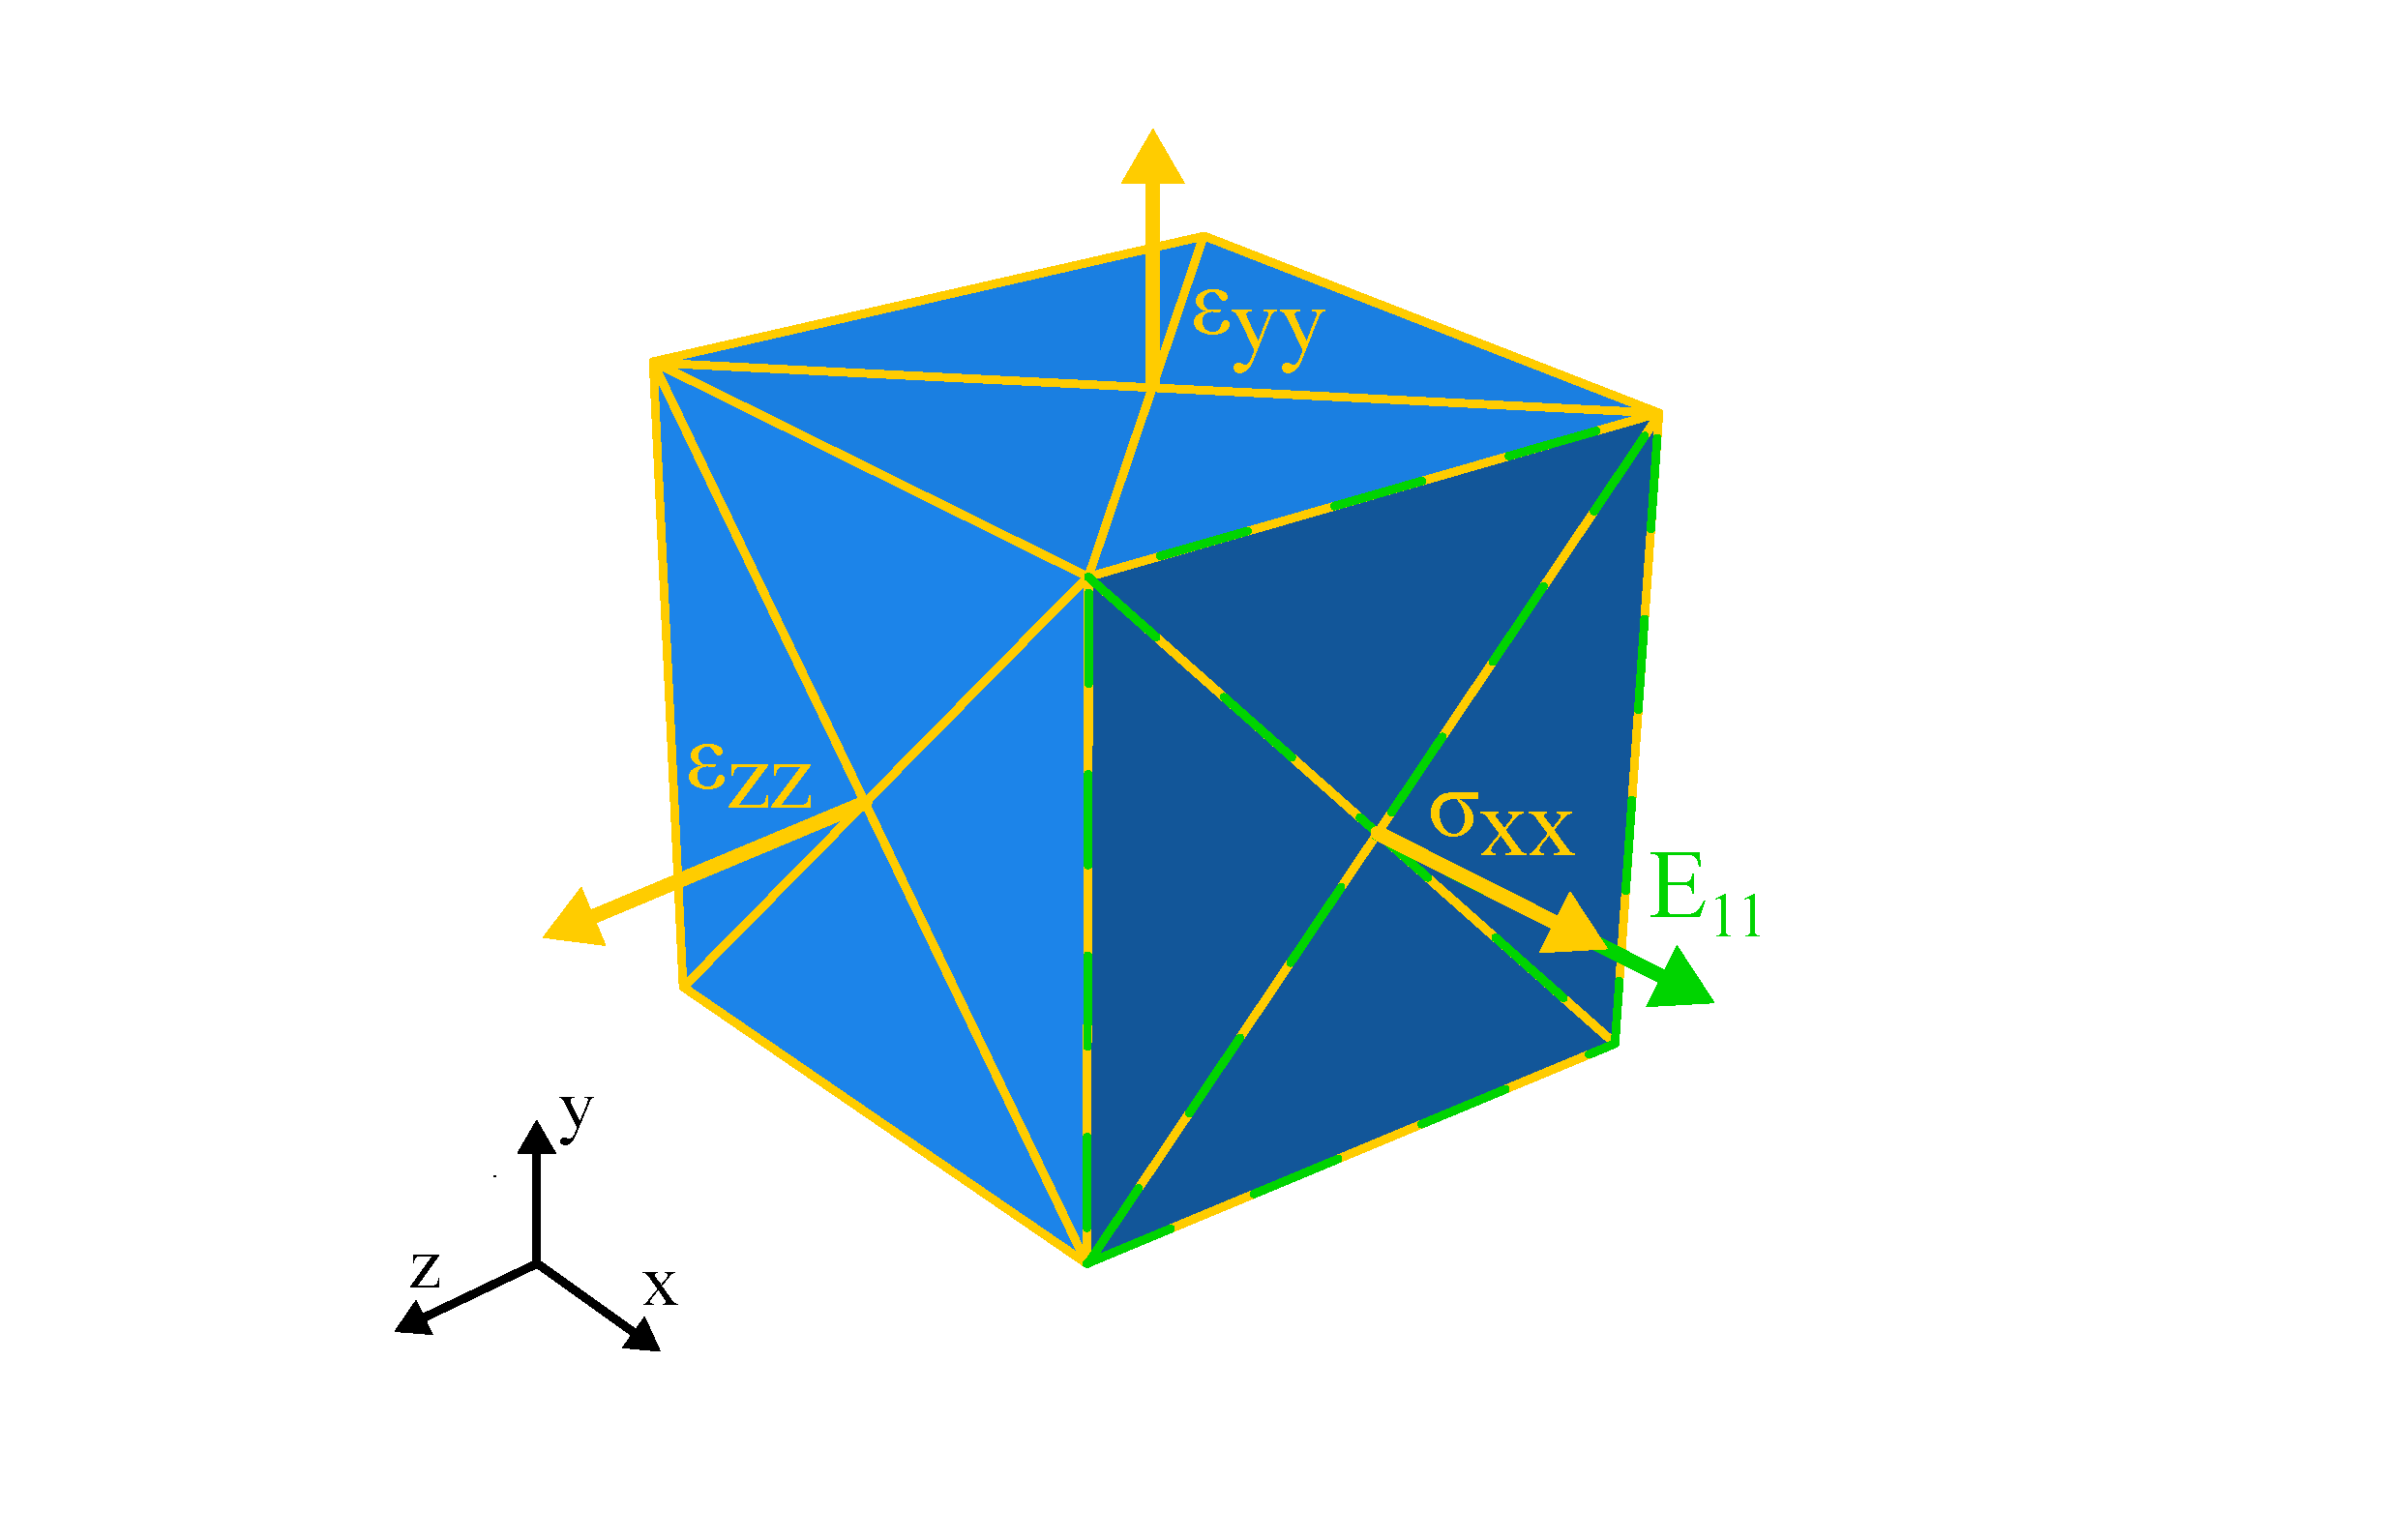
\includegraphics[width=0.7\textwidth]{cube_loading_plain_white_new.pdf}
    \caption{Illustration of exemplary load case E11 acting on the front surface in $xx$-direction (represented in green) with its exemplary evaluated stress and strain reactions $\sigma_{xx}, \varepsilon_{yy}$ and $\varepsilon_{zz}$ on the surfaces (represented in yellow)}
    \label{fig:evaluationMeasurements}
\end{figure}

\subsection{Load parameters and load reactions}\label{subsec:loadParameters}
For the optimisation process we use data from \acrshort{md} simulations as inputs. This data are referenced as \emph{reference data} in the following. They contain stress and strain components for all time steps during the loading process, in all normal and shear directions. Thus, we can register different trends of loading with the corresponding reactions.
We split the reference data into \emph{load parameters} and \emph{\acrlong{rlr}}. The load parameters define the quantitative values of the prescribed load case. 
Since we defined the load cases identical to the ones in the \acrshort{md} simulations, we can process the data from the load parameters directly. 
If the load case is known, we can easily extract the load parameters from the reference data and transfer them into the \acrshort{fe} model. A detailed description of the load application in \name{Abaqus} can be found in \autoref{sec: preprocessing}. 
The \acrlong{rlr} represent the material response during the \acrshort{md} simulation. From this, we extract the stress and strain components according to the chosen \acrlong{er}. 
We neglect the remaining stress and strain components, since they contain little information about the material behaviour.
To perform the inverse parameter identification, we need corresponding data from the \acrshort{fe} simulation.
In the way described in \autoref{sec: optimisationCode}, we can read out stress and strain components in all directions. Similar to the \acrlong{rlr} we extract the values corresponding to the \acrlong{er}. These values are called \emph{\acrlong{olr}}. \\
\indent In \autoref{tab: testSeries} the test series with their loading conditions are listed.
In the verification and validation studies we apply linear strain up to a maximum value of 20 \%. For the validation studies we use different mixing ratios which show different mechanical behaviours. As a preparation for studies with cyclic loading, we investigate a pure tensile strain following the first quarter sinus period over time with a maximum amplitude of 15 \% strain. With this loading trajectory, we study the optimisation behaviour for non-linear loading parameters.
We reuse this load parameters, and apply them as a shear strain in load case G12. Since in the previous tests always the load case E11 is used, we test the script performance for another load case.
To obtain more information about the material behaviour, we combine the load cases of E11 and G12 in one optimisation. 
As a last study we investigate one and a half period of a sinusoidal loading for a tensile load case in $xx$-direction. We use amplitudes of 1 \%, 5 \% and 8 \%. Important to notice is that the previously introduced load parameters proceed in a wide strain range. Assuming that the material starts to plastify quite fast, the majority of the loading steps are located in the plastic domain of the material. Conversely, the load parameters contain only little information about the elastic material behaviour. 
Through the use of load parameters with small amplitudes, we try to get a larger proportion of data points in the elastic domain.
In \autoref{sec: verification} the issue about this unequal distribution in the material domains becomes clear.    

\begin{table}[H]
    \centering
    \renewcommand{\arraystretch}{1.3}
    \caption{Overview of test series with corresponding loading conditions, materials and evaluated reactions}
    \label{tab: testSeries}
    \begin{tabular}{L{0.17\textwidth}C{0.08\textwidth}C{0.13\textwidth}C{0.15\textwidth}C{0.13\textwidth}C{0.17\textwidth}}
    \toprule
    \multirow{2}{0.17\textwidth}{\textbf{Test series}} & \multirow{2}{0.08\textwidth}{\centering \textbf{Load case}} & \multicolumn{2}{C{0.28\textwidth}}{\textbf{\ Load parameters}} &  \multicolumn{1}{C{0.13\textwidth}}{\multirow{2}{0.13\textwidth}{\centering \textbf{Mixing ratio}}} &\multirow{2}{0.17\textwidth}{\centering \textbf{Evaluated reaction}} \\ \cmidrule{3-4}
    & &\textbf{Trajectory} & \textbf{Amplitude} & & \\  \midrule
    Verification & E11 & Linear & 20\% & 6:3 & \(\sigma_{xx}, \varepsilon_{yy}, \varepsilon_{zz}\)\\\hline
    Validation I & E11 & Linear & 20\% & 4:3 & \(\sigma_{xx}, \varepsilon_{yy}, \varepsilon_{zz}\)\\ \hline
    Validation II& E11 & Linear & 20\% & 6:3 & \(\sigma_{xx}, \varepsilon_{yy}, \varepsilon_{zz}\)\\ \hline
    Validation III& E11 & Linear & 20\% & 8:3 & \(\sigma_{xx}, \varepsilon_{yy}, \varepsilon_{zz}\)\\ \toprule
    \multirow{2}{0.15\textwidth}{Pure tensile strain} & E11 & Sinus (\(\frac{1}{2} \pi\)) & 15\% & 6:3 & \(\sigma_{xx}, \varepsilon_{yy}, \varepsilon_{zz}\)\\ 
            &   &           &   && \\ \hline
    Simple shear strain  & G12 & Sinus (\(\frac{1}{2}\pi\)) & 15\% & 6:3 & \(\sigma_{xy}\)\\ \hline
    \multirow{2}{0.15\textwidth}{Tensile \& Shear strain} & E11 & Sinus (\(\frac{1}{2}\pi\)) & 15\% & 6:3 & \(\sigma_{xx}, \varepsilon_{yy}, \varepsilon_{zz}, \sigma_{xy}\)\\ 
                            & G12 &       &      &     \\ \hline
    \multirow{2}{0.15\textwidth}{Cyclic tensile strain} & E11 & Sinus (\(3\pi\)) & 1\%  & 6:3 & \(\sigma_{xx}, \varepsilon_{yy}, \varepsilon_{zz}\)\\ 
                &     &       & 5\%  &  & \(\sigma_{xx}, \varepsilon_{yy}, \varepsilon_{zz}\)\\ 
                &     &       & 8\%  & & \(\sigma_{xx}, \varepsilon_{yy}, \varepsilon_{zz}\)\\ \bottomrule
    \end{tabular}
    
\end{table}



\section{Error Calculation}\label{sec: errorCalculation}
For a representative value including all necessary data we use the \acrshort{rmse}, which is explained in \autoref{subsec: RMSE}. Therefore, we use \autoref{eq: multiRMSE}, and insert the \acrlong{rlr} and the \acrlong{olr} as data sets.
The extraction of the load reactions is described in \autoref{sec: optimisationCode}.
We compute the deviations of the \acrlong{olr} at each load step. \autoref{fig: erroPlot} displays this procedure for an exemplary set of \acrlong{rlr} and \acrlong{olr}. Here $\sigma_{xx}$ is the selected \acrlong{er}. For every load step LS their corresponding \acrfull{rlr} $\sigma_{\scriptscriptstyle\text{LS}}^{\scriptscriptstyle\text{RLR}}$ and \acrfull{olr} $\sigma_{\scriptscriptstyle\text{LS}}^{\scriptscriptstyle\text{OLR}}$ are logged. The blue arrow highlights their deviation $\Delta\sigma_{\scriptscriptstyle\text{LS}}$ for one exemplary load step, according to \autoref{eq: EMDifference}. 
As described in \autoref{subsec:loadParameters}, the distribution of the data points is unfavourable for the determination of the elastic parameters. 
To support the script in finding the elastic parameters, we applied a weight of 100 at the data point in the elastic domain, i.e. below 1 \% strain. This is done via an array $\boldsymbol{w}$ which entries are one except the first entry $w_{\scriptscriptstyle\text{1}}$. Formally, the applied weights have the inverse unit of the evaluated load reaction, i.e. for stress load reactions, $[w_{\text{LS}}] = \text{MPa}^{-1}$ would be the correct unit for the related weights.
According to \autoref{eq: mse}, we calculate the mean value of the weighted arrays.
The resulting value is called \emph{\acrfull{mse}} for one \acrlong{er}. We compute $\text{MSE}_{\sigma}$ or $\text{MSE}_{\varepsilon}$ for every selected \acrlong{er}. 

\begin{figure}[H]
    \centering
    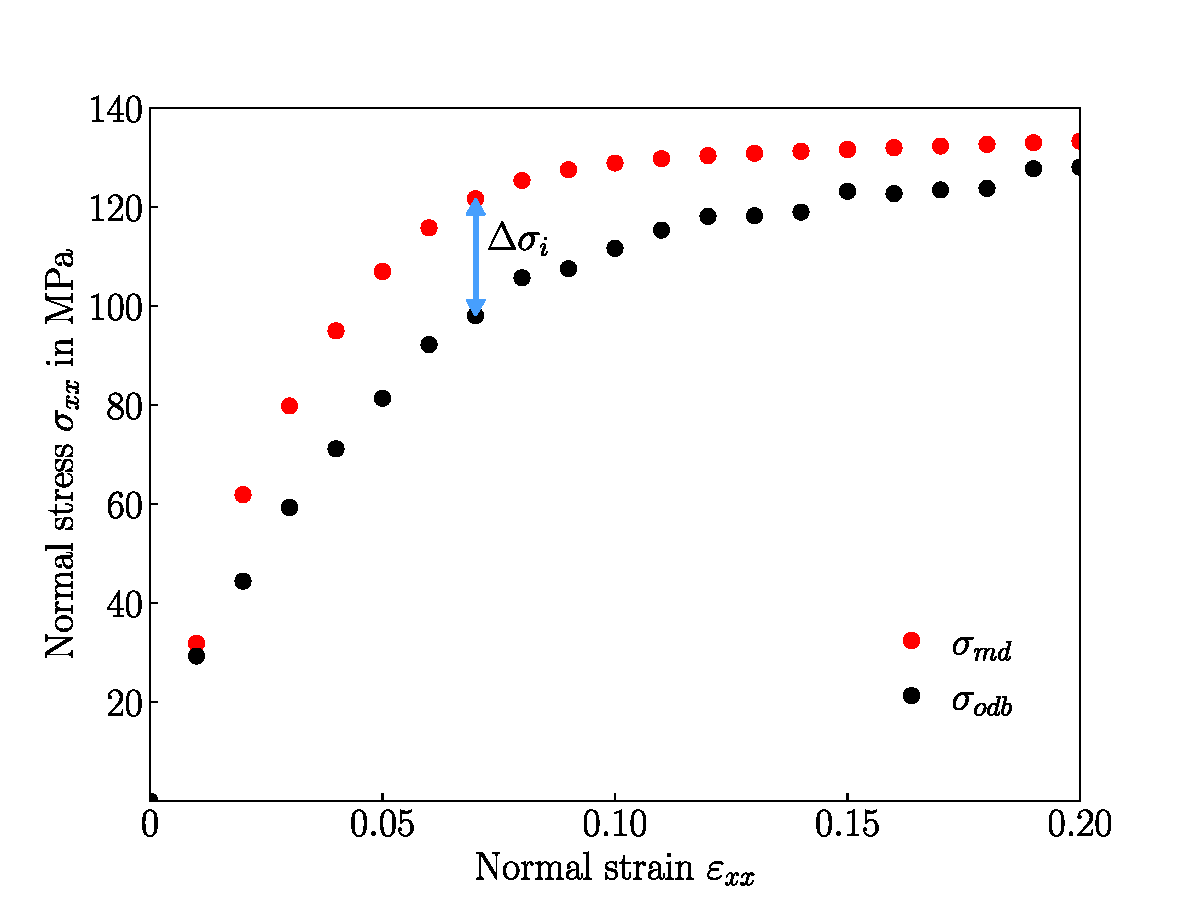
\includegraphics[width = 0.65\textwidth]{error_plot.pdf}
    \caption{Exemplary \acrlong{rlr} $\sigma^{\scriptscriptstyle\text{RLR}}$ and \acrlong{olr} $\sigma^{\scriptscriptstyle\text{OLR}}$ with visualization of error calculation}
    \label{fig: erroPlot}
\end{figure}
XX FIGURE ANPASSEN

\begin{gather}
    \label{eq: EMDifference}
    \Delta\sigma_{\scriptscriptstyle\text{LS}} = \sigma_{\scriptscriptstyle\text{LS}}^{\scriptscriptstyle\text{RLR}} - \sigma_{\scriptscriptstyle\text{LS}}^{\scriptscriptstyle\text{OLR}} \hspace{2cm}
    \Delta\varepsilon_{\scriptscriptstyle\text{LS}} = \varepsilon_{\scriptscriptstyle\text{LS}}^{\scriptscriptstyle\text{RLR}} - \varepsilon_{\scriptscriptstyle\text{LS}}^{\scriptscriptstyle\text{OLR}}\\
    \label{eq: mse}
    \text{MSE}_{\sigma} = \frac{\displaystyle\sum_{\text{LS}} w_{\scriptscriptstyle\text{LS}} (\Delta\sigma_{\scriptscriptstyle\text{LS}}^2)}{\displaystyle\sum_{\text{LS}}w_{\scriptscriptstyle\text{LS}} } \hspace{2cm}
    \text{MSE}_{\varepsilon} = \frac{\displaystyle\sum_{\text{LS}} w_{\scriptscriptstyle\text{LS}} (\Delta\varepsilon_{\scriptscriptstyle\text{LS}})^2}{\displaystyle\sum_{\text{LS}}w_{\scriptscriptstyle\text{LS}}}
\end{gather}

For the tensile load case for example, we must perform this for the \acrlong{er} $\sigma_{xx}, \varepsilon_{yy} \text{ and } \varepsilon_{zz}$. 
In order to construct a single error value of these \acrshort{mse}s, we must ensure a common scale. Otherwise, their influence on the overall error may vary significantly.
In general, the \acrshort{mse}s of \acrlong{eer} are much smaller than the ones from \acrlong{esr}, such that loading dependent weights $w_{\sigma}$ and $w_{\varepsilon}$ are introduced. 
The exact weights depend on the load case and the used load parameter set.
From the weighted \acrshort{mse} we construct the \acrshort{rmse} as shown in \autoref{eq: rmse}. 
Since the code is able to process multiple load cases in one optimisation process, we can calculate the \acrshort{rmse} for every load case and apply associated weights $w_{\scriptscriptstyle\text{LC}}$. Additionally, multiple load parameters sets (LP) can be processed, which leads to \acrshort{rmse} values for every load parameter set with the weight $w_{\scriptscriptstyle\text{LP}}$. 
As stated in \autoref{eq: error}, we assemble the individual \acrshort{rmse}s in a double sum over the load cases and the load parameter sets. This \benennung{Error} is the value we return the numerical optimisation algorithm. In the following sections we have a closer look at the implementation of this minimisation process. 

\begin{gather}
    \label{eq: rmse}
        \text{RMSE} = \sqrt{\frac{\displaystyle\sum_{\text{ESR}} w_{\sigma} \cdot \text{MSE}_{\sigma} + \displaystyle\sum_{\text{EER}} w_{\varepsilon} \cdot \text{MSE}_{\varepsilon}}{N_\text{ESR} + N_\text{EER}}} \\
        \label{eq: error}
    \text{Error} = \sum_{\text{LP}} \sum_{\text{LC}} w_{\scriptscriptstyle\text{LP}} w_{\scriptscriptstyle\text{LC}} \cdot \text{RMSE}_{\scriptscriptstyle \text{LC}, \text{LP}} \\
        N_\text{ESR}: \text{Number of \acrlong{esr}} \nonumber\\
    N_\text{EER}: \text{Number of \acrlong{eer}} \nonumber
\end{gather}


\section{Preprocessing} \label{sec: preprocessing}
Before starting with the optimisation process, we need preprocessing steps to create a working \name{Abaqus} model with the required properties. The user-defined properties are transferred in an input-file. \autoref{tab: inputParameterTable} lists an extract of this file, containing only parameters relevant for the optimisation process.
\begin{table}[H]
    \centering
    \caption{Input parameters for optimisation process}
    \label{tab: inputParameterTable}
    \renewcommand{\arraystretch}{1.1}
    \begin{tabular}{L{0.2\textwidth}C{0.2\textwidth}C{0.15\textwidth}C{0.1\textwidth}C{0.1\textwidth}}
    \toprule
    \textbf{Input parameter} & \textbf{Directions} & \textbf{Category} & \textbf{Data format} & \textbf{Unit} \\ \midrule
    Young's modulus & – & value    & array  & MPa \\ 
                & – & minimum  & scalar & MPa \\ 
                & – & maximum  & scalar & MPa \\ \hline
    Poisson's ratio  & – & value    & array  & –   \\ 
                & – & minimum  & scalar & –   \\ 
                & – & maximum  & scalar & –   \\ \hline
    Yield stress  & – & value    & array  & MPa \\ 
                & – & minimum  & scalar & MPa \\ 
                & – & maximum  & scalar & MPa \\ \hline
    \multirow{2}{0.2\textwidth}{Alpha, beta, gamma} & – & value    & array  & –   \\ 
                    & – & minimum  & scalar & –   \\ 
                    & – & maximum  & scalar & –   \\ \hline
    Load parameters & – & filename & string & –   \\ 
                    & – & weight   & scalar & –   \\ \hline
    Load case & \multirow{2}{0.2\textwidth}{E11, E22, E33, G12, G23, G13} & active & boolean    & – \\ 
            &                               & weight & scalar & – \\ \hline
    Stress evaluation & \multirow{2}{0.15\textwidth}{$xx$, $yy$, $zz$, $xy$, $yz$, $xz$} & active & boolean   & – \\ 
                    &                        & weight & scalar & – \\ \hline
    Strain evaluation & \multirow{2}{0.15\textwidth}{$xx$, $yy$, $zz$, $xy$, $yz$, $xz$} & active & boolean  & – \\ 
                    &                        & weight & scalar & – \\ \hline
    Load weighting & \multirow{4}{0.2\textwidth}{normal stress, normal strain, shear stress, shear strain} & weight & scalar & – \\ 
    &&&& \\
    &&&& \\
    &&&& \\\bottomrule
    \end{tabular}
    
\end{table}

The input file contains more parameters for different namings, which are neglected here. In attaachment XX the whole input file is included. 
The user has multiple options to configure the optimisation process. It is possible to test multiple initial value combinations for the material parameters calling the script once. In \autoref{tab: inputParameterTable} this is visible in the column \benennung{Data format} of the values of all material parameters. This function is important to validate the optimisation results with varying input values. \\
\indent In \autoref{fig: flowchart} the complete structure of the code is depicted. The white boxes show the individual steps referred to in the text in italics. The coloured boxes represent the performed loops. 
The upper part belongs to the preprocessing, which starts with the step \benennung{Read input file}.
In this step all entries from the input-file are extracted. 
For every material parameter the script writes an array of initial values. Then the code loops over all array entries at a time to extract one initial value for each parameter. Therefore, the entries with the same index add up to one initial value combination which is visualised in \autoref{tab:material_combinations}. As a consequence all arrays need to be of same length. For all initial value combinations the code creates a new \acrfull{mdb} in \name{Abaqus}, and a new folder structure to set the working directory and store the results.




\begin{table}[h!]
    \centering
    \caption{Loop conditions in preprocessing}
    \label{tab:loop_conditions}
    \begin{subtable}[t]{0.45\textwidth}
        \centering
        \renewcommand{\arraystretch}{1.1}
        \caption{Arrangement of initial value combination of material parameters}
        \label{tab:material_combinations}
        \begin{tabular}{L{0.31\textwidth}|C{0.08\textwidth}C{0.08\textwidth}C{0.08\textwidth}C{0.08\textwidth}C{0.08\textwidth}}
            \toprule
            \multirow{2}{0.31\textwidth}{\textbf{Material Parameter}} & \multicolumn{5}{c}{\textbf{Combination}} \\
            \cmidrule(lr){2-6}
             & \textbf{1} & \textbf{2} & \textbf{3} & \textbf{4} & \textbf{5} \\ \midrule
            $E$ & $E_1$ & $E_2$ & $E_3$ & $E_4$ & $E_5$ \\ \hline
            $\nu$ & $\nu_1$ & $\nu_2$ & $\nu_3$ & $\nu_4$ & $\nu_5$ \\\hline
            $\sigma_0$ & $\sigma_{0_1}$ & $\sigma_{0_2}$ & $\sigma_{0_3}$ & $\sigma_{0_4}$ & $\sigma_{0_5}$ \\\hline
            $\alpha$ & $\alpha_1$ & $\alpha_2$ & $\alpha_3$ & $\alpha_4$ & $\alpha_5$ \\\hline
            $\beta$ & $\beta_1$ & $\beta_2$ & $\beta_3$ & $\beta_4$ & $\beta_5$ \\\hline
            $\gamma$ & $\gamma_1$ & $\gamma_2$ & $\gamma_3$ & $\gamma_4$ & $\gamma_5$ \\ 
            \bottomrule
        \end{tabular}
    \end{subtable}  
    \hfill
    \begin{subtable}[t]{0.45\textwidth}
        \centering
        \renewcommand{\arraystretch}{1.17}
        \caption{Model creation for load case and parameter combinations}
        \label{tab:model_creation}
        \begin{tabular}{L{0.25\textwidth}|C{0.2\textwidth}C{0.35\textwidth}}
            \toprule
            {\textbf{Model}} & \textbf{Load case} &  \textbf{Load parameters} \\ \midrule
            Model 0 & E11 & Data set 1 \\ \hline
            Model 1 & E11 & Data set 2 \\\hline
            Model 2 & E11 & Data set 3 \\\hline
            Model 3 & G12 & Data set 1 \\\hline
            Model 4 & G12 & Data set 2 \\\hline
            Model 5 & G12 & Data set 3 \\
            \bottomrule
        \end{tabular}
    \end{subtable}    
\end{table}

Afterwards we start the first loop with \benennung{Create model}. As discussed in \autoref{sec: FEMBasics} we model a cube with size 1x1x1. We mesh the cube with 6x6x6 elements. Because of the regular geometry, we work with hexagonal structured elements to keep the model simple. The number of elements is a compromise between a coarse mesh for fast computation and a minimum number to avoid convergence errors. Although we use a hyperelastic material in our optimisation process, we first have to build the model with elastic material. We apply isotropic behaviour and define Young's modulus and Poisson ratio as the initial values. \\
\indent The elastic material is necessary due to the usage of EasyPBC in the step \benennung{Create job}. We use the load case defined in the input file to create a job. As discussed in \autoref{subsec: EasPBC}, we use EasyPBC for the automatic construction of \acrshort{pbc}. Aside from that, we adopt the generated load application corresponding to the load case. Since the load acts on a reference point, connected to the whole loaded surface, a homogeneous load contribution is ensured.
However, the settings from EasyPBC contain some default values, we adjust in the step \benennung{Modify properties}. EasyPBC applies for every load case a uniform displacement with a standard fixed value, while we want to study the complete loading process. For a correct comparison of the loading reactions we have to evaluate the stresses and strains in the \acrshort{fe} simulation at the same step sizes as in the \acrshort{md} simulation. In \name{Abaqus} we can solve this issue by creating an amplitude to apply the load gradually (see \autoref{fig:amplitudemenu}). Therefore, we enter the load parameters as an amplitude at certain time steps. For the time steps we use consecutive numbers, since the steps sizes are already defined through the amplitude. The value in the boundary condition editor is then set to one because this only defines the factor by which the amplitude is multiplied (see \autoref{fig:bcmenu}). Afterwards we modify the increment settings. EasyPBC automatically creates increments with fixed size and without non-linear geometry effects. In order to avoid convergence errors, we use automatic incrementation. Especially in the first load steps, we observe large deformations. If we try to resolve such large deformations in one incrementation step, \name{Abaqus} runs into convergence errors. With automatic incrementation \name{Abaqus} can adapt the number of increments per load step dynamically dependent of the current deformation. The non-linear geometry effects have to be considered for the same reason. In the last step of preprocessing we store the model in a dictionary. We use this dictionary later to call the models for the optimisation. We perform the preprocessing for all prescribed load cases, highlighted in green in the flowchart. Furthermore, the purple area visualises the loop over the load parameters. This leads to individual models for every load case and every load parameter set, which is visualised in \autoref{tab:model_creation}.

\begin{figure}[H]
    \centering
    % --- Subfigure (a)
    \begin{subfigure}[t]{0.35\textwidth}
        \centering
        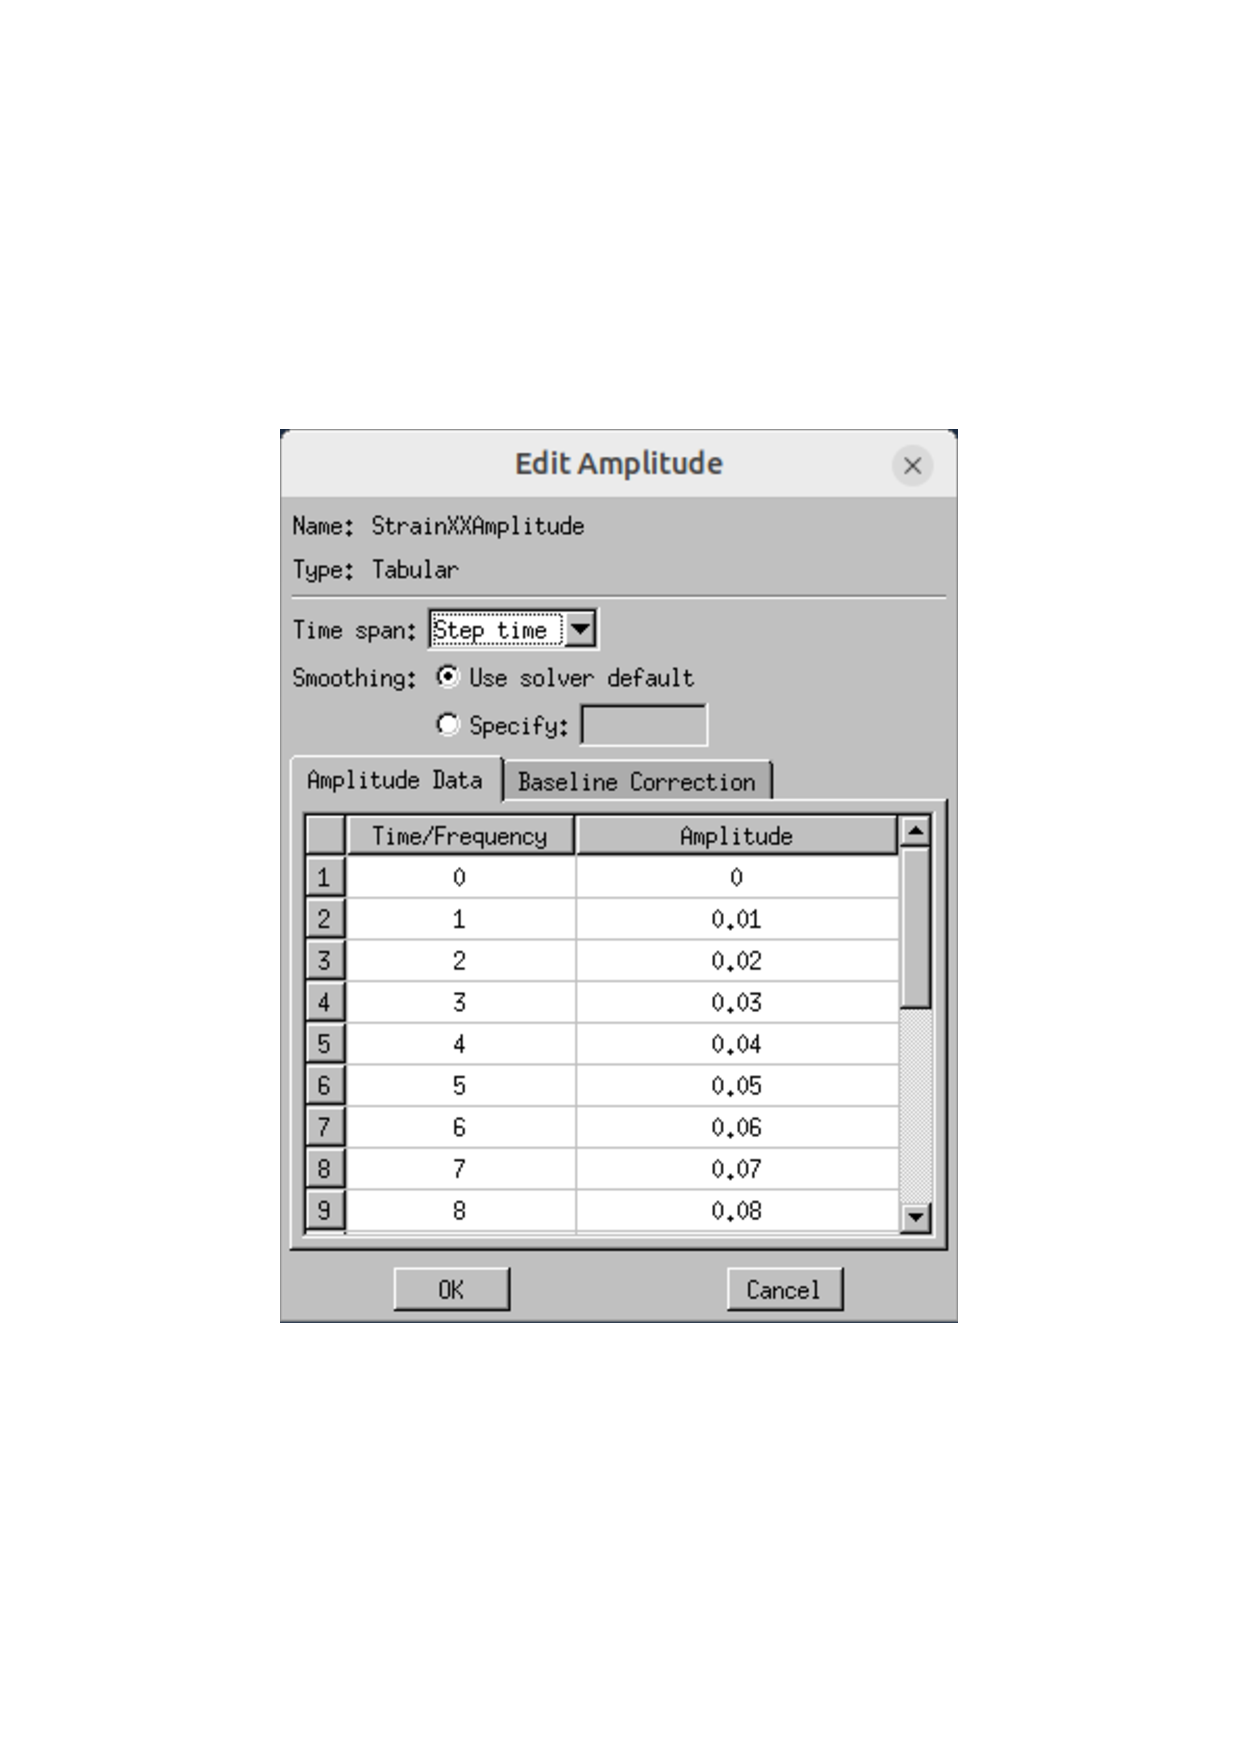
\includegraphics[width=\linewidth]{Amplitude.pdf}
        \vfill{}
        \caption{ Definition of load amplitude in \name{Abaqus}} % eigene (a)-Caption
        \label{fig:amplitudemenu}
    \end{subfigure}
    \hspace{0.08\textwidth}
    % --- Subfigure (b)
    \begin{subfigure}[t]{0.35\textwidth}
        \centering
        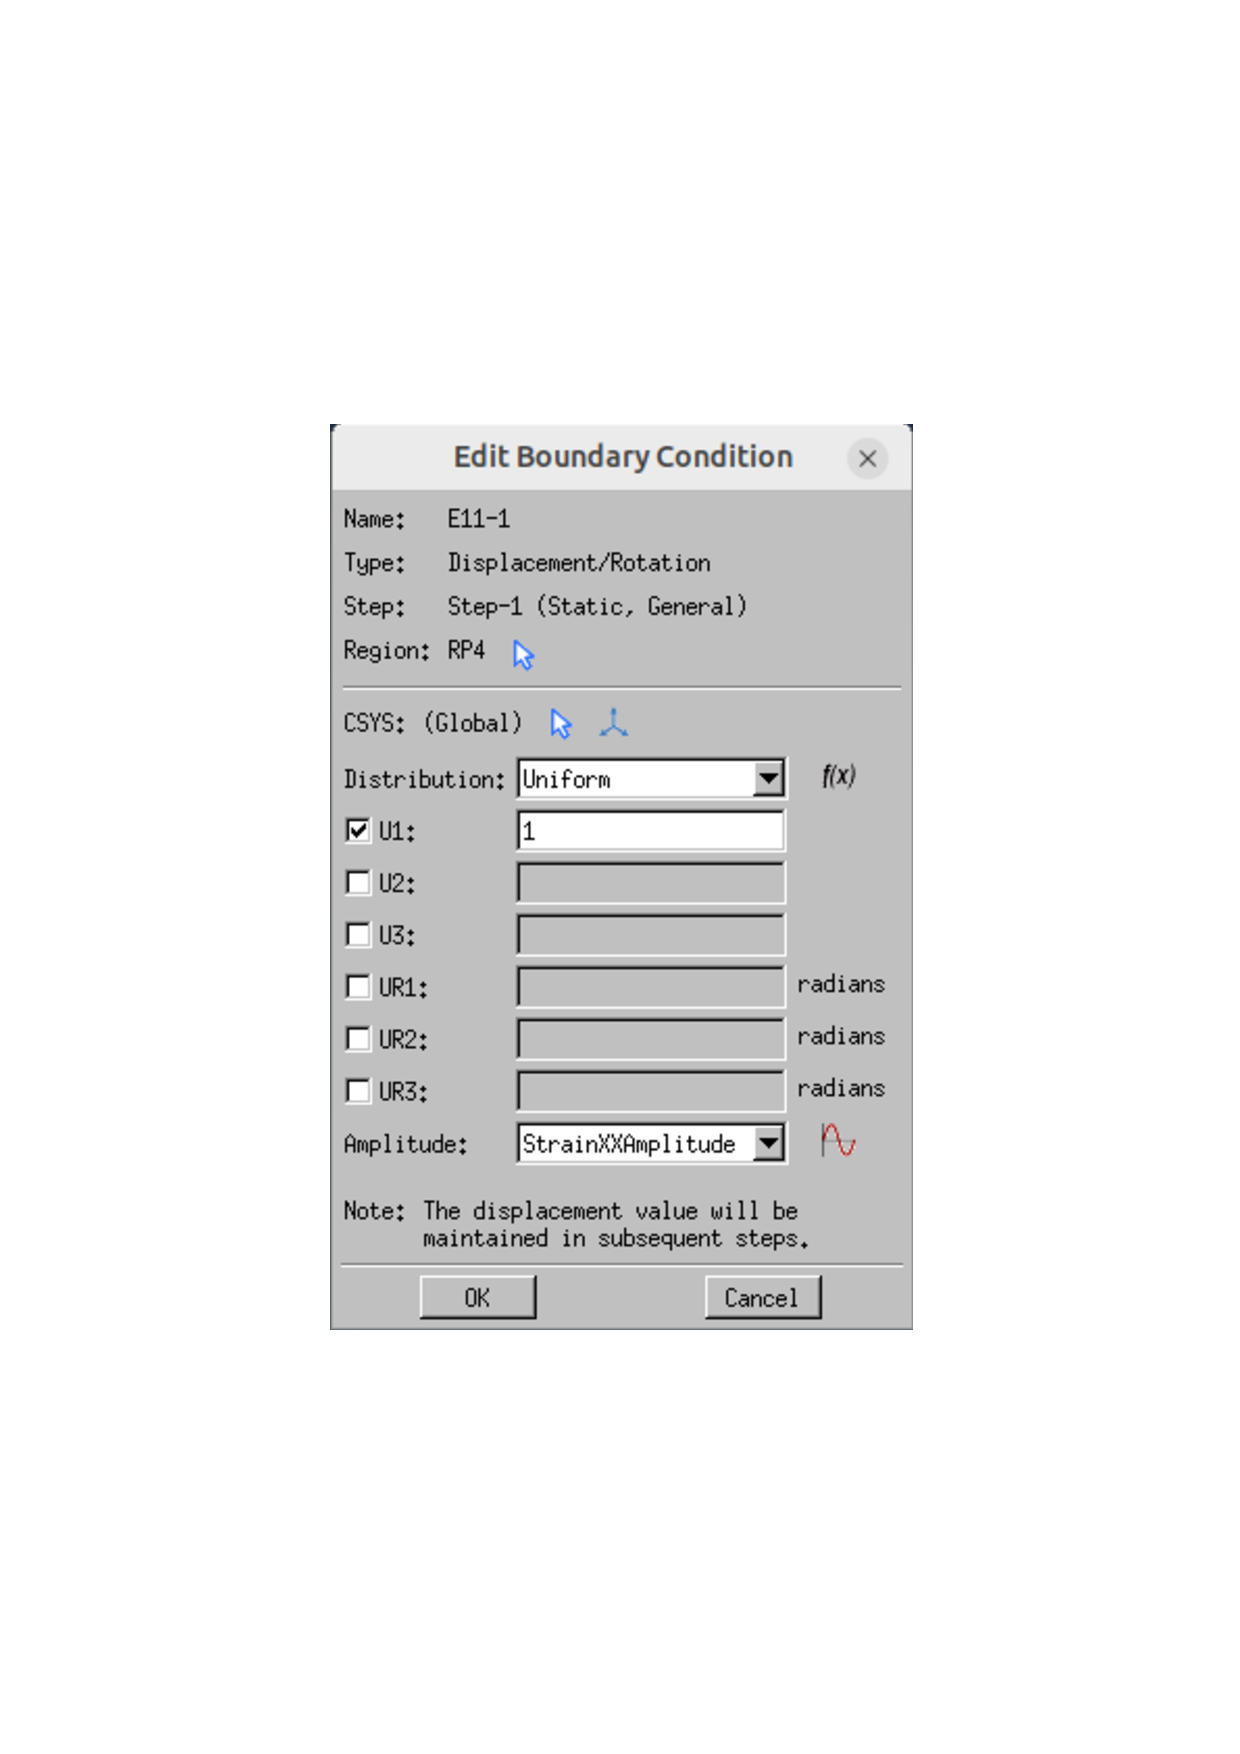
\includegraphics[width=\linewidth]{BC.pdf}
        \caption{Boundary condition menu in \name{Abaqus}}
        \label{fig:bcmenu}
    \end{subfigure}

    \caption{Loop conditions in preprocessing}
    \label{fig:abaqus_settings}
\end{figure}

\section{Optimisation process} \label{sec: optimisationCode}

\begin{figure}[H]
    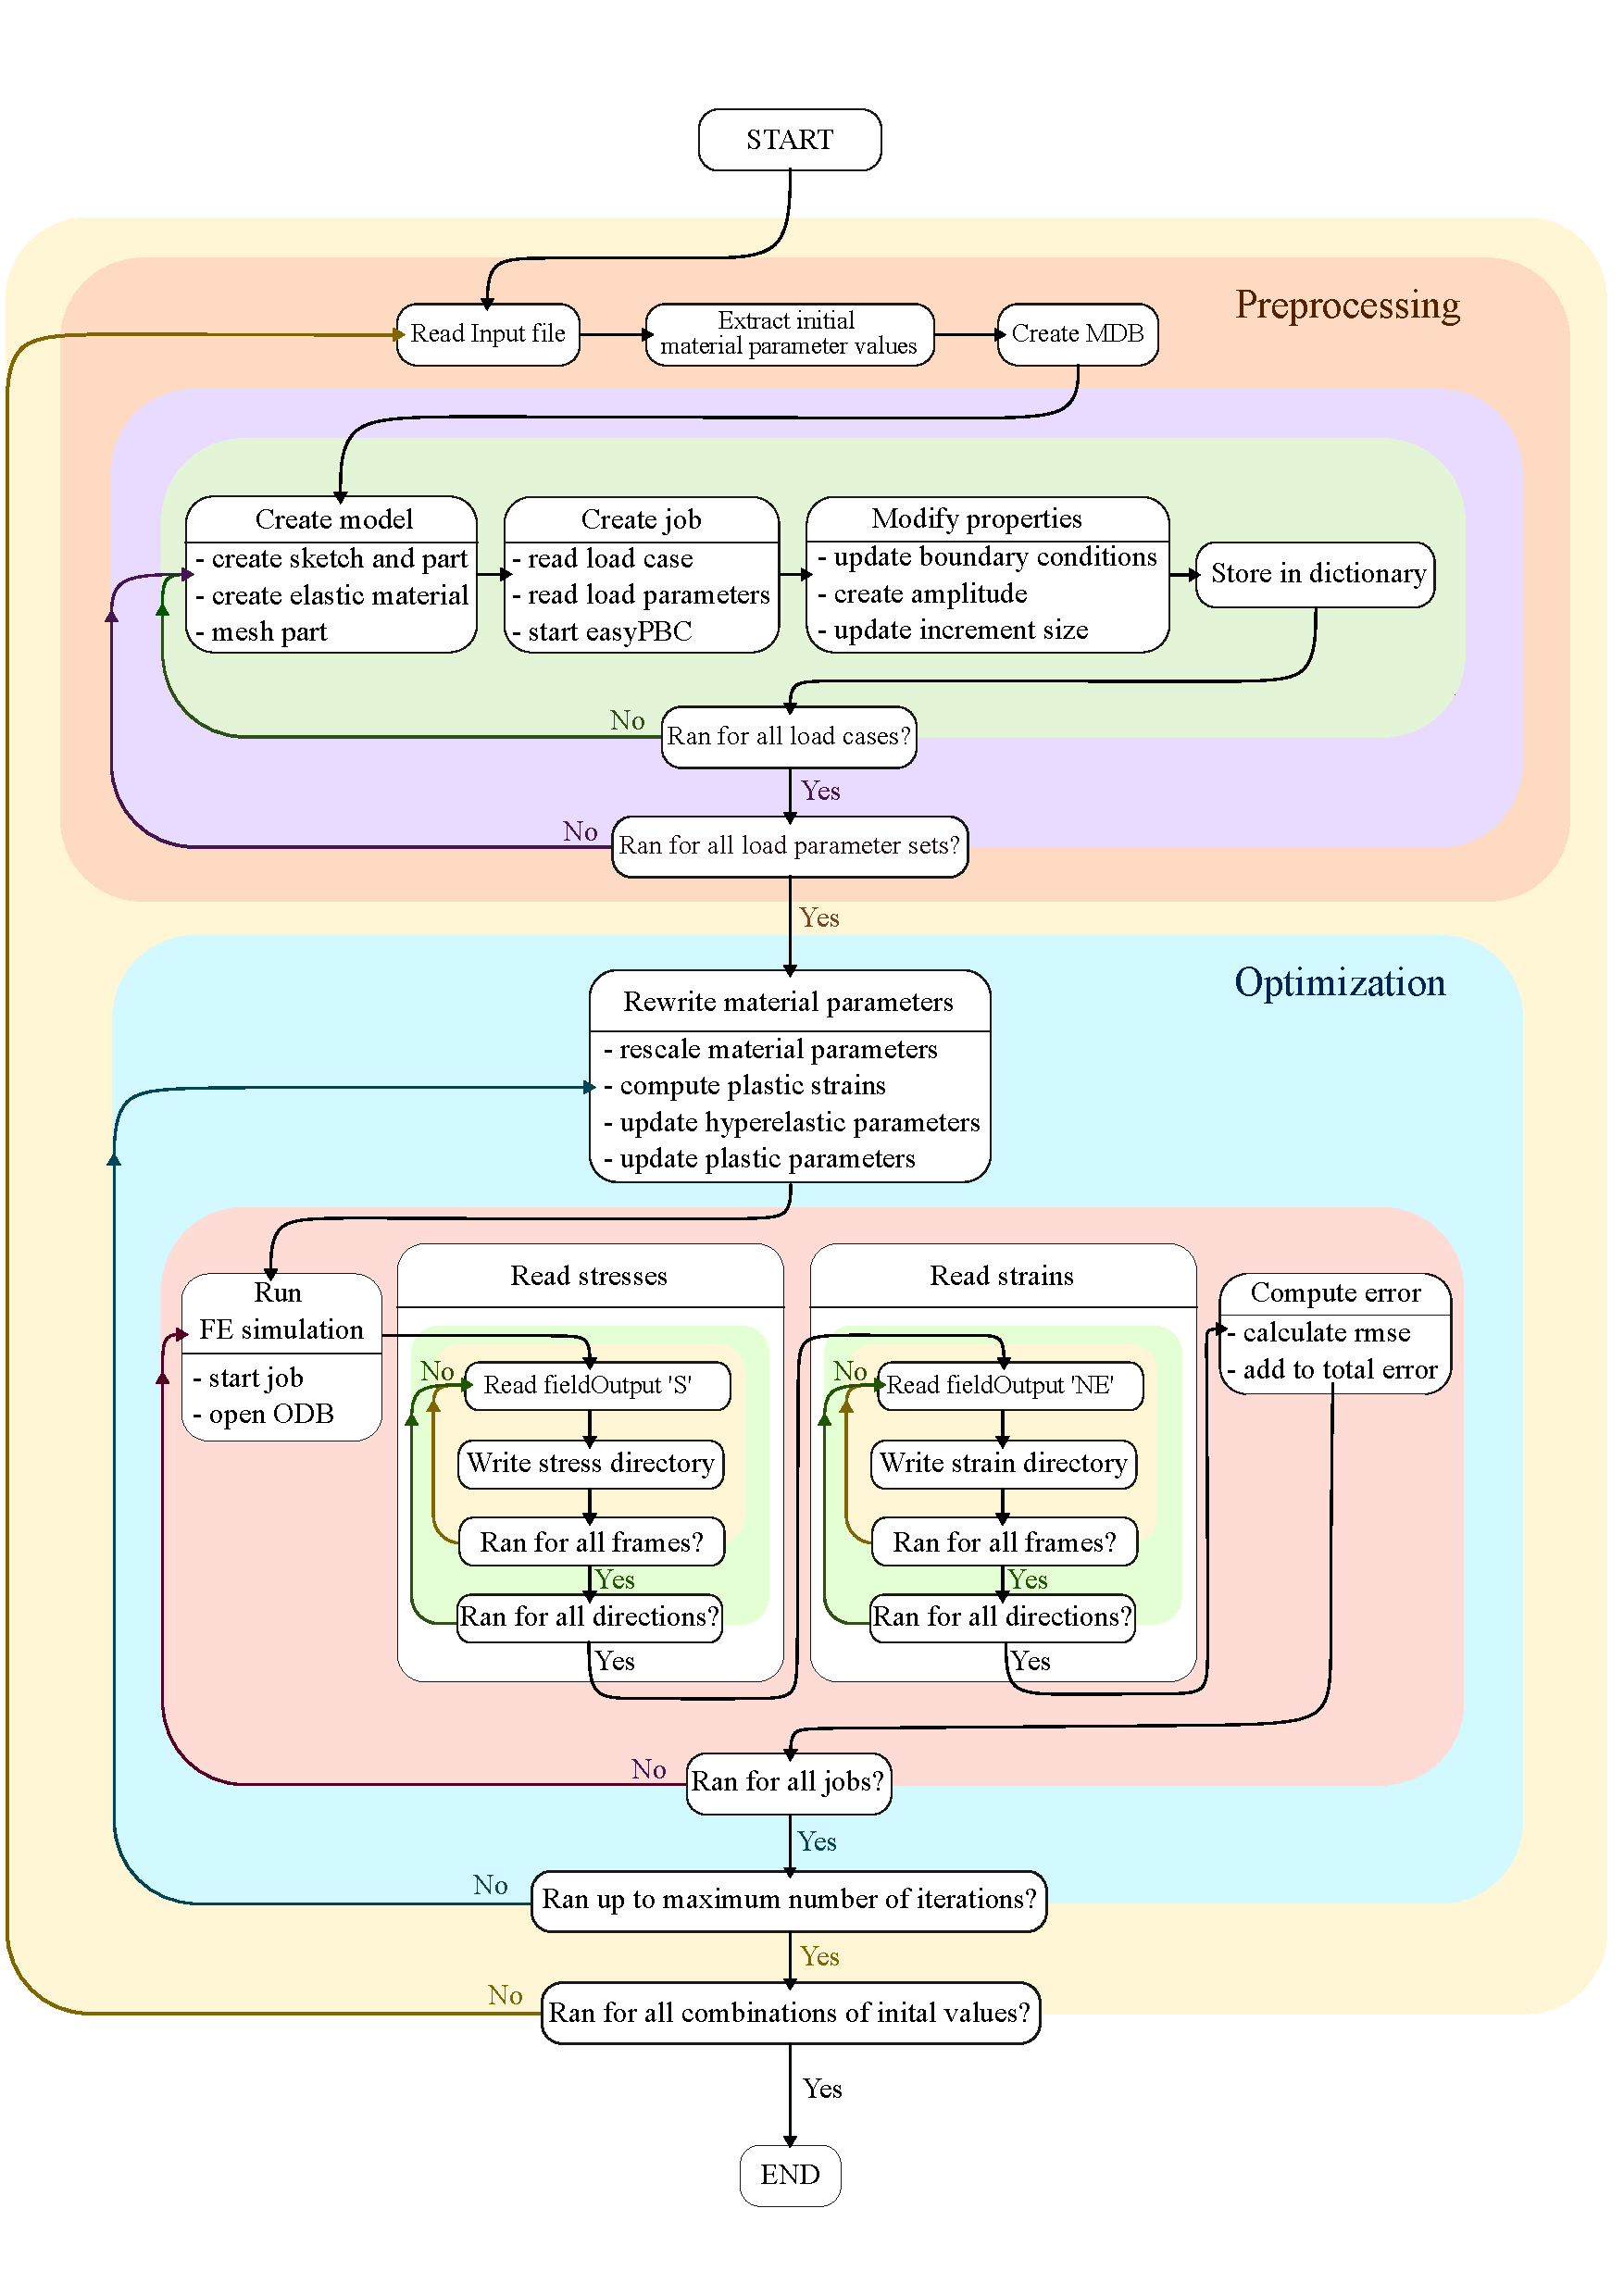
\includegraphics[width = 1.0\textwidth]{complete_flowchart_new.pdf}
    \caption{Flowchart code}
    \label{fig: flowchart}
\end{figure}

\begin{table}[h!]
\centering
\renewcommand{\arraystretch}{1.2}
\caption{Input parameters for SciPy minimize function}
\label{tab: minimizeFunctionInput}
\begin{tabular}{L{0.15\textwidth}|L{0.2\textwidth}C{0.12\textwidth}L{0.4\textwidth}}
\toprule
\textbf{Parameter} & \textbf{Content} & \textbf{Data format} & \textbf{Explanation} \\
\midrule
Objective function & Optimisation function & -- & Function whose scalar value should be minimized \\ \hline

Initial guess & Material parameters & array & Scaled initial values for the optimisation parameters \\\hline

\multirow{2}{0.15\textwidth}{Additional arguments}
 & Cube parameters & object & Model information from input file \\
 & Load parameters & dictionary & Load parameters from MD-simulations \\
 & Work directory & string & Path to store results \\
 & Evaluation counter & scalar & Counter for the performed function evaluations \\ \hline

method & Nelder-Mead & -- & Numerical algorithm \\\hline

bounds & Limits for material parameter & array & Upper and lower boundary values for every optimisation parameter \\\hline

maxiter & Number of iterations & scalar & Maximum number of iterations  as termination criterion\\
\bottomrule
\end{tabular}
\end{table}

In the following section, we describe the optimisation process. We start the process by calling the Scipy-minimize function. We pass this function various parameters, listed in \autoref{tab: minimizeFunctionInput}. The minimize function itself calls our self-written optimisation function, where the evaluation takes place. The initial guess stores an array with start values for all parameters that should be optimised. Additionally, we pass information about the models that we created in the preprocessing and the load parameters. We use all models created in the purple box for one optimisation call.
We start the process with the step \benennung{Rewrite material parameters} for all models. Since they all describe the same material, we write the same values for every model. For the minimisation computation, optimisation parameters are scaled in the bounds from zero to one. To rewrite the values in the models, we have to rescale them first. Then we can use the rescaled parameters to compute the values for the hardening-function with the formula for VOCE-hardening (\autoref{eq: voce}). In the following we remove the elastic material and substitute it with a hyperelastic material which is suitable for high non-linear deformations. Therefore, we have to convert the Young's modulus and the Poisson's ratio into the hyperelastic parameters $C_{10}$ and $D_1$ via the relations
\begin{gather}\label{eq: elasticParams}
    C_{10} = \frac{E}{4(1+ \nu)} \hspace{1.5cm}
    D_1 = \frac{6(1-2\nu)}{E}.
\end{gather}

Now we can update all material values. In the next steps we handle the models successively. We start the job of the first model to perform the \name{Abaqus} analysis and open the resulting \acrshort{odb} in \benennung{Run FE-simulation}. With step \benennung{Read stresses} the evaluation begins. We do this by reading the 'FieldOutput' variable 'S' and write the data in a stress directory. Since we need stress-values at all steps defined by the amplitude, we read out every frame from the \acrshort{odb}. One frame corresponds with one step in the loading process. Additionally, we loop over all directions ($xx$, $yy$, $zz$, $xy$, $yz$, $xz$). The same procedure is done for the strain values in \benennung{Read strains}. Here it is important to read out the correct strain variable 'NE' (nominal strain). For hyperelastic materials, \name{Abaqus} uses the logarithmic strain ('LE') as standard value. Because of its logarithmic scaling, we cannot compare them to the reference data. Then we store all values for all frames and directions in a dictionary, similar as for the stresses. Now we have collected all required data to perform the step \benennung{Compute error}. We do this in the way described in \autoref{sec: errorCalculation}. For a better structure of the code this part is outsourced in a separate function. We call this function and pass the stress and strain directories as well as the corresponding load parameters. Then the computation runs and the function returns the \acrshort{rmse} for this job. Multiplied with its corresponding weights for its load case and load parameters we add this value to the total error value. Now we restart the red loop by starting the FE-simulation for the next job which is visualised in the red box in the flowchart. Once all the jobs are processed, and we computed the total error value, we return it to our minimisation function. Through the internal Nelder-Mead algorithm the error is reduced and it returns the corresponding material parameters. Now one optimisation iteration is performed and it starts again. In the flowchart, the loop is visualised with the blue box. This process will run until our defined number of maximum iterations is reached or convergence is reached. When the changes in the error value are very small, the internal convergence criterion is reached and the algorithm stops.


\section{Data storage} \label{sec: dataStorage}

To evaluate the optimisation process at the end, parameter values need to be recorded during the preprocessing and the optimisation process. This is the only way to ensure that the values of all iterations are saved, since the variable values are rewritten in every new iteration. In the preprocessing, we extract the input file with the current initial value combination. All files created from \name{Abaqus} like the CAE, \acrshort{odb} and the job-files are stored in a subfolder. In the optimisation part, multiple functions are called after the step \benennung{Compute error} to store the current variable values. The material parameters for every iteration are stored. In addition, we store multiple interim results during the error calculation. For every job the weighted \acrshort{mse}s are stored for every iteration, so that the impact and evolution of every evaluated reactions can be understood. To track the impact of the applied weights, all \acrshort{rmse} values are stored individually and weighted. In addition, we store the total error, which is the sum of all weighted \acrshort{rmse}s of one iteration. Finally, we have one file each for the material parameters, \acrshort{mse}s, \acrshort{rmse}s, and the total errors. All these files are handled in the same way. After the computation of the total error, all files are opened and the variable values of the current iteration are stored in a new line. The stress and strains are stored in separate files for each iteration. We create for each job a subfolder, where its stress and strain values are stored. For one iteration, a file is created which contains the stress and strain dictionaries from the steps \benennung{Read stress} and \benennung{Read strain}. This leads to as many files as iterations were performed for every job. At the end of the optimisation process, we store the final message returned from the Scipy.minimize function. \name{Python} automatically sends a message where the cause of termination is stated. This message becomes important if the algorithm stops before the maximum number of iterations is reached. Then we can reproduce whether this happens because the convergence limit is reached or a numerical error occurred. The described procedure to store the data is done for every initial value combination separately.

\begin{table}[H]
    \centering
    \renewcommand{\arraystretch}{1.2}
    \caption{Overview of the performed tests with corresponding input parameters}
    \label{tab:storageData}
    \begin{tabular}{L{0.3\textwidth}|C{0.1\textwidth}L{0.5\textwidth}}
    \toprule
   \textbf{Stored parameters} & \textbf{Data format} & \textbf{Explanation}\\ \midrule
   Input parameters & JSON & Copy of the input file with current initial value combination\\ \hline
   Material parameters & CSV & Table with all material parameters for each evaluation\\\hline
   weighted \acrshort{mse} & CSV & File per job with weighted \acrshort{mse} per evaluation \\\hline
   \acrshort{rmse} & CSV & File with \acrshort{rmse} per job, each stored alone, with weight for load case, and weight for load parameters \\\hline
   Total error & CSV & Total error after each evaluation \\\hline
   Optimised load reactions & CSV & File per job with all optimised load reactions in one evaluation \\\hline
   Scipy.minimize message & TXT & Final message about the termination status of the scipy-function\\
    \bottomrule
    \end{tabular}
    
\end{table}

MINIMIZE FUNCTION IN FLOWCHART INTEGRIEREN


% All data are stored in csv-format.

% - store results
% - welche results
% - material parameters for every iteration
% - rmse value for every iteration for every job (weighted and unweigthed)
% - total eror for every iteration
% - input file with inital value combination
% - abaqus model
% - stress and strain values for evaluated reactions for every iteration in sperate file
% - all in csv files
% - easy to handle 
% - kann gut direkt angeschaut werden und grobe einschätzung machen
% - leicht auszulesen
% - reference data
% - rmse message (message of scipy function) --> falls abbruch wg convergence error oder so 


        
    % eventuell plot format noch anpassen, wie voce und RMSE plot sinnvoll einbauen?
    % sind RMSE plots überhaupt notwendig bei validation?
    % strain-strain plot bei verification einfügen
    
    \chapter{Results}\label{chap: results}

    In this chapter the results from different test cases presented in section XX will be evaluated. First, we discuss the verification results to understand the general behavior of the optimization process. In the next step we validate the optimization performance using different data sets. 
    Finally, we present the results of the cyclic load cases.

    
    \section{Verification}\label{sec: verification}

    In this section, we discuss the results of the data set used for the verification of our optimization process. To evaluate the quality of the optimization process, we define characteristic quantities and investigate their evolution. 
    Noch den load case kurz aufschreiben.


    \begin{figure}[H]
		\centering
        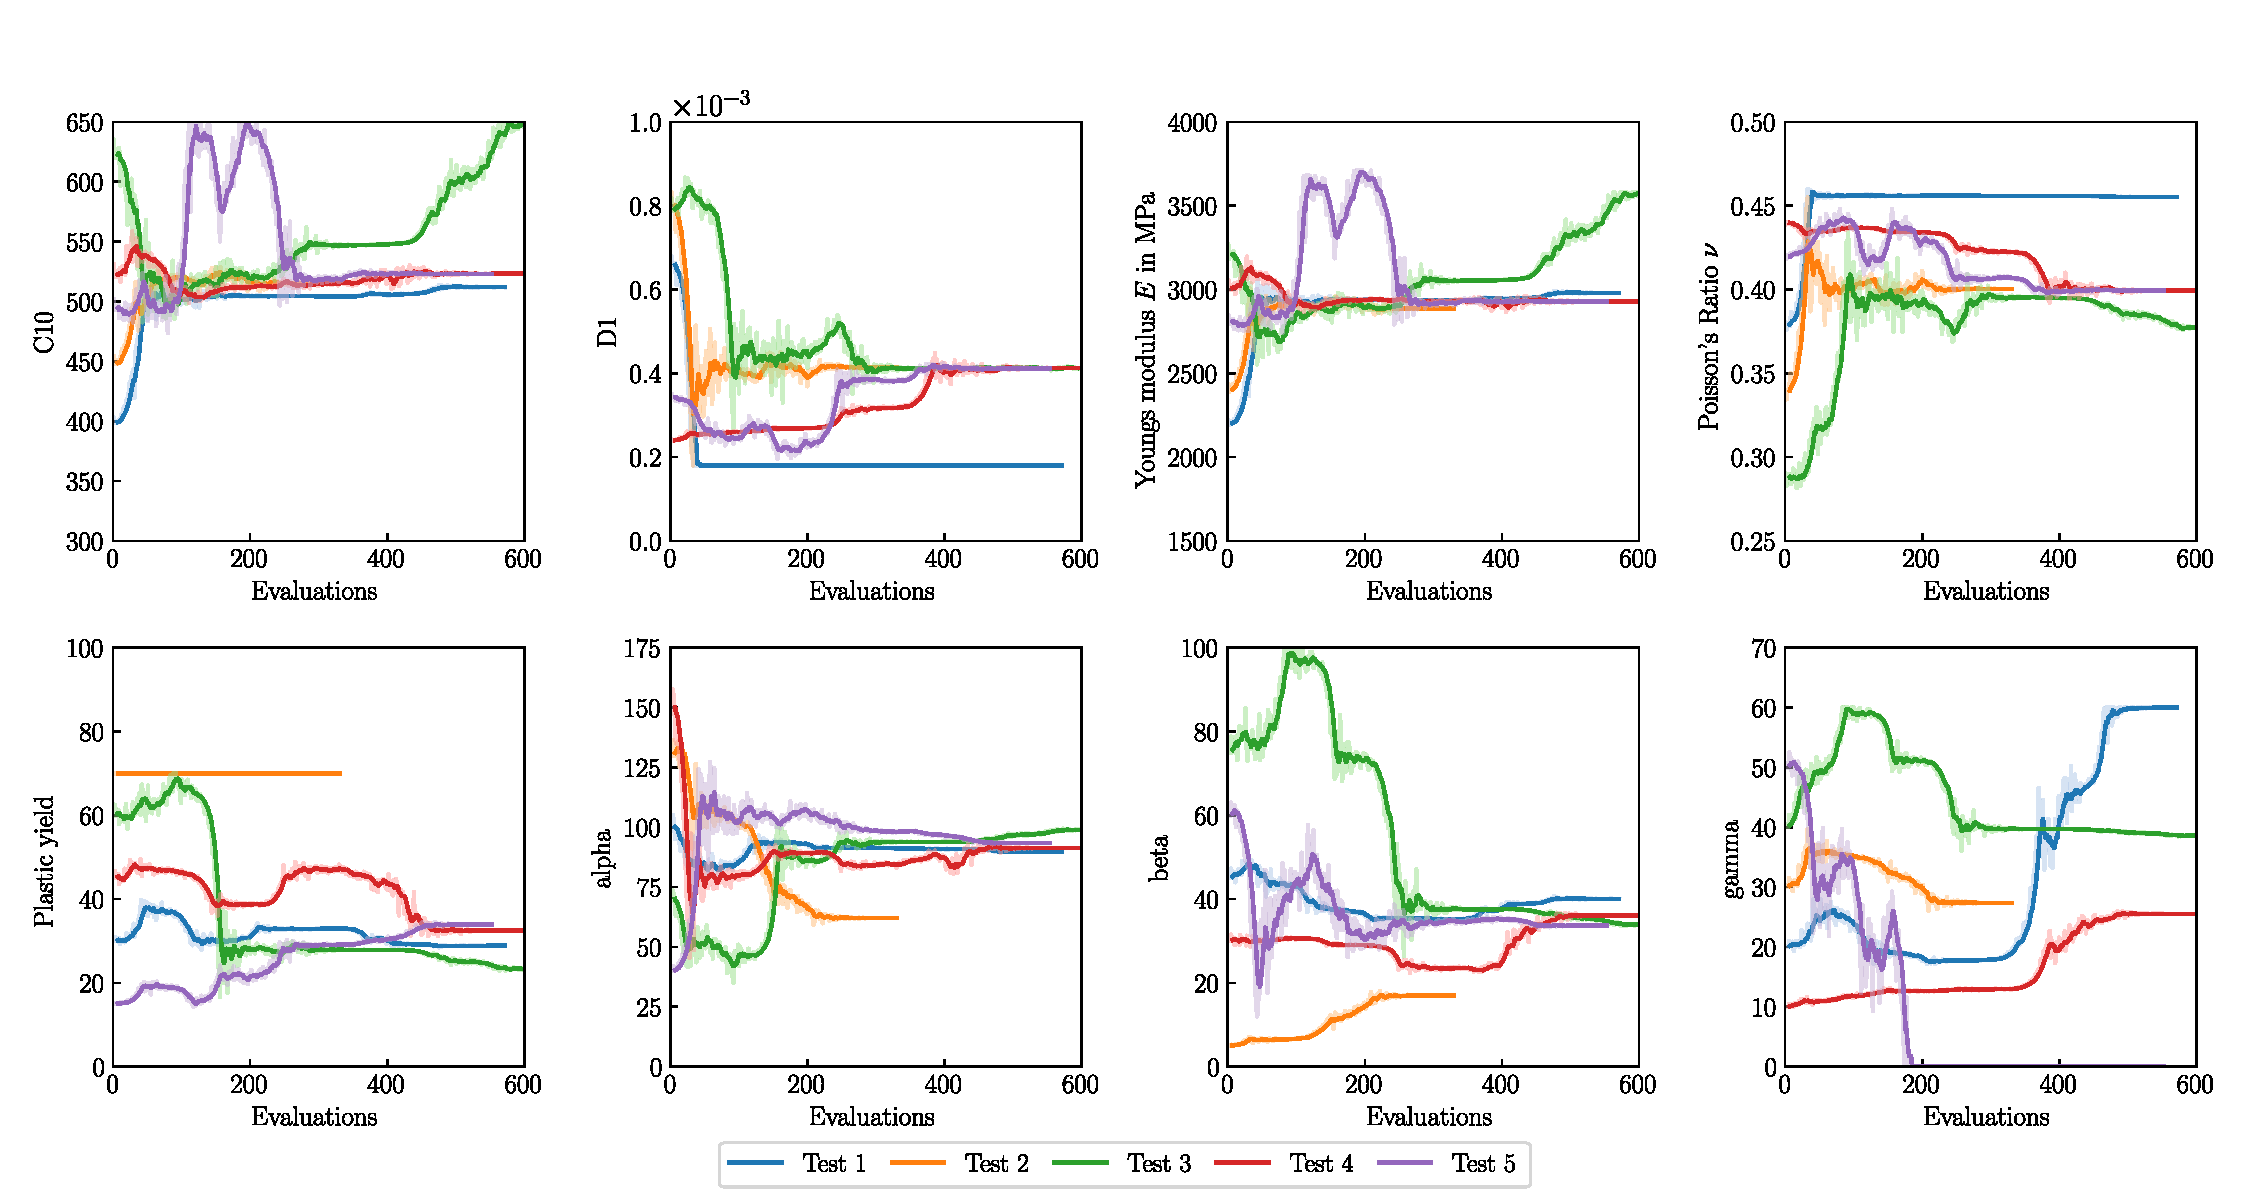
\includegraphics[width=0.7\textwidth]{verify_material_params.pdf}
		\caption{optimization progress of material parameters}
		\label{fig:materialparameters}
	\end{figure}
    As process quantities we log the evolution of the material parameters during the optimization. Since these are our input parameters we performed multiple tests with varying parameter combinations to evaluate the stability of our program. The results are presented in \ref{fig:materialparameters}. In the first row the elastic material parameters are presented. For a better understanding, we transformed the hyper-elastic parameters \(C10\) and \(D1\) into Young's modulus \(E\) and Poisson ratio \(\nu\). In the second row the plastic material parameters are presented. For elastic and plastic parameters we can observe convergence for every parameter combination. However, the converged solutions differ from each other for most of the combinations. 
    For a detailed discussion of possible reasons we separate between elastic and plastic material behavior. Since our tested material shows an elastic response only up to the second data point, there might be not enough optimization points to find an unique solution for the elastic material parameters. Nevertheless, we have to investigate other characteristic quantities to ensure our assumption and understand the influence of the plastic parameters. In \autoref{fig:progress stress-strain curve} the progress of the stress-strain curve in normal direction during one exemplary test together with the target curve from the MD simulation is presented. The optimized curve matches the target curve after only  \(25 \%\) of the evaluations. Since the stress-strain curve is one of our target data this progress indicates a correct optimization behavior of our algorithm. To support this assumption the final stress-strain curves of the test series are depicted in \autoref{fig:final stress-strain curves}. Despite the high variance of the final material parameters, the stress-strain curves all matches the target data for the stress-strain curve in normal direction. Because of this deviation we depicted the influence of the parameters on the trend of the VOCE-hardening curve shown in \autoref{fig:Parameter influence on VOCE-hardening curve}. The parameter alpha has the greatest impact on the shape of the curve, while a variety of \(50\%\) in the parameter gamma has hardly any visible effect. This leads to a high flexibility in adjusting the shape of the curve and as a consequence to multiple possible parameter combinations to fit the target curve. To support our assumption we check the quality of the optimization result by plotting the progress of the root mean squared error (RSME) for all the tests in \autoref{fig:rmse progress}. We observe that a common minimum RMSE value is reached in all optimization runs, indicating that the results are of equivalent quality. 
    The results of this verification tests lead to some states about the quality of the optimization algorithm. The results of the stress-strain data show a good match of the optimized curve with the target data for every test which is confirmed by the RMSE. In contrast we observe a high variance in final the material parameters found by the algorithm. These results suggest that the algorithm can generally find parameter values to match the target data. However, the variance in these optimal parameters shows that multiple parameter combinations lead to the same quality of result. This behavior may be due to the relatively large number of optimization parameters compared to the dimension of the target data. To verify this assumption we reduced the number of material parameters. Since only the first point of the target data lies in the elastic domain, we fixed the elastic material behavior and computed them directly from the data of the first point. Then we tested this new configuration of the algorithm with the current target data and two other data sets.


    \begin{figure}[H]
        \centering
        \subfigure[evolution of stress-strain curve]{
            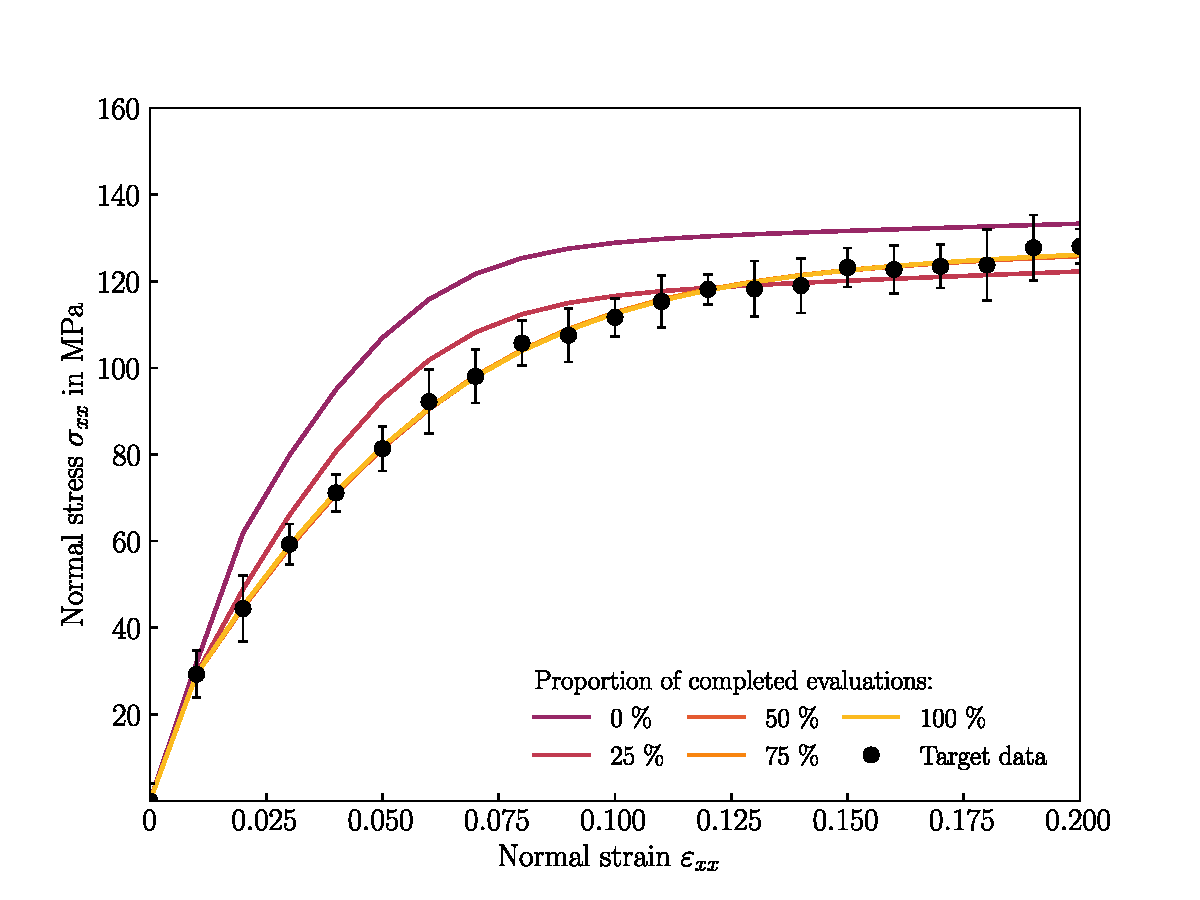
\includegraphics[width=0.47\textwidth]{verfiy_stress_strain_progress.pdf}
            \label{fig:progress stress-strain curve}
        }
        \subfigure[final stress-strain curves]{     
            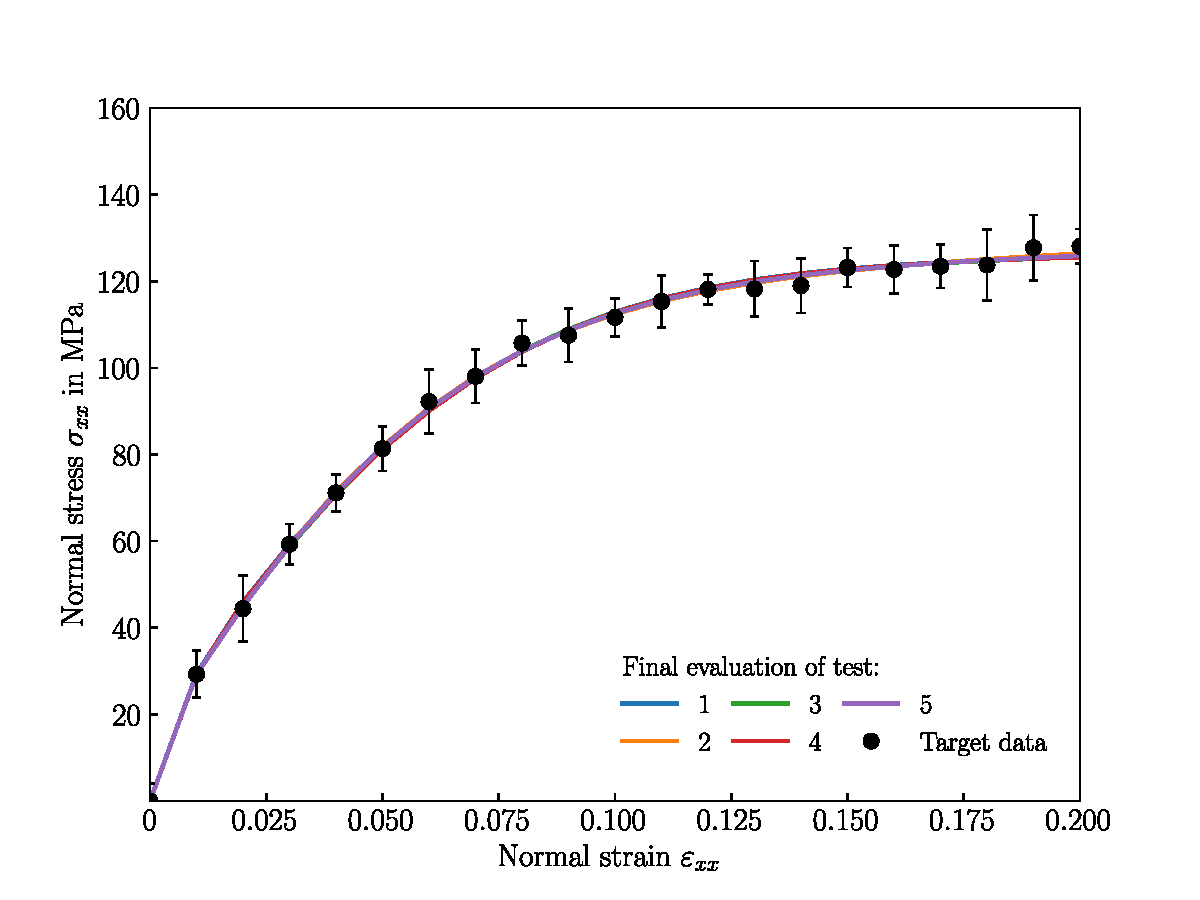
\includegraphics[width=0.47\textwidth]{verify_stress_strain_combined.pdf}
            \label{fig:final stress-strain curves}
        }
        \caption{a) evolution of the stress-strain curves during optimization for exemplary test, b) final stress-strain curves for complete test study}
        \label{fig:complete}
    \end{figure}


   
   \begin{figure}[H]
		\centering
        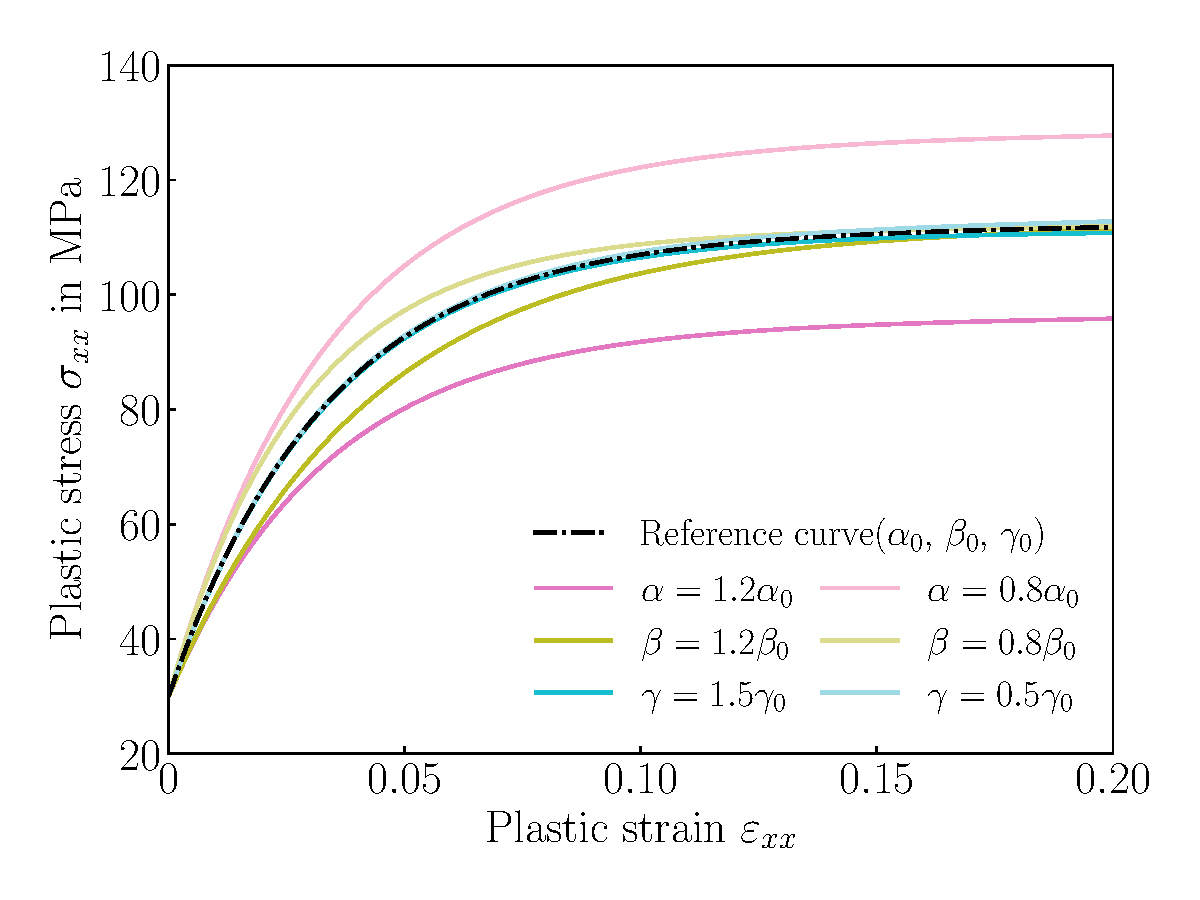
\includegraphics[width=0.5\textwidth]{voce_curve.pdf}
		\caption{parameter influence on voce-hardening curve}
		\label{fig:Parameter influence on VOCE-hardening curve}
	\end{figure}
    PICTURES with Krümmung und Steigung --> parameters to characterize curve

    \begin{figure}[H]
		\centering
        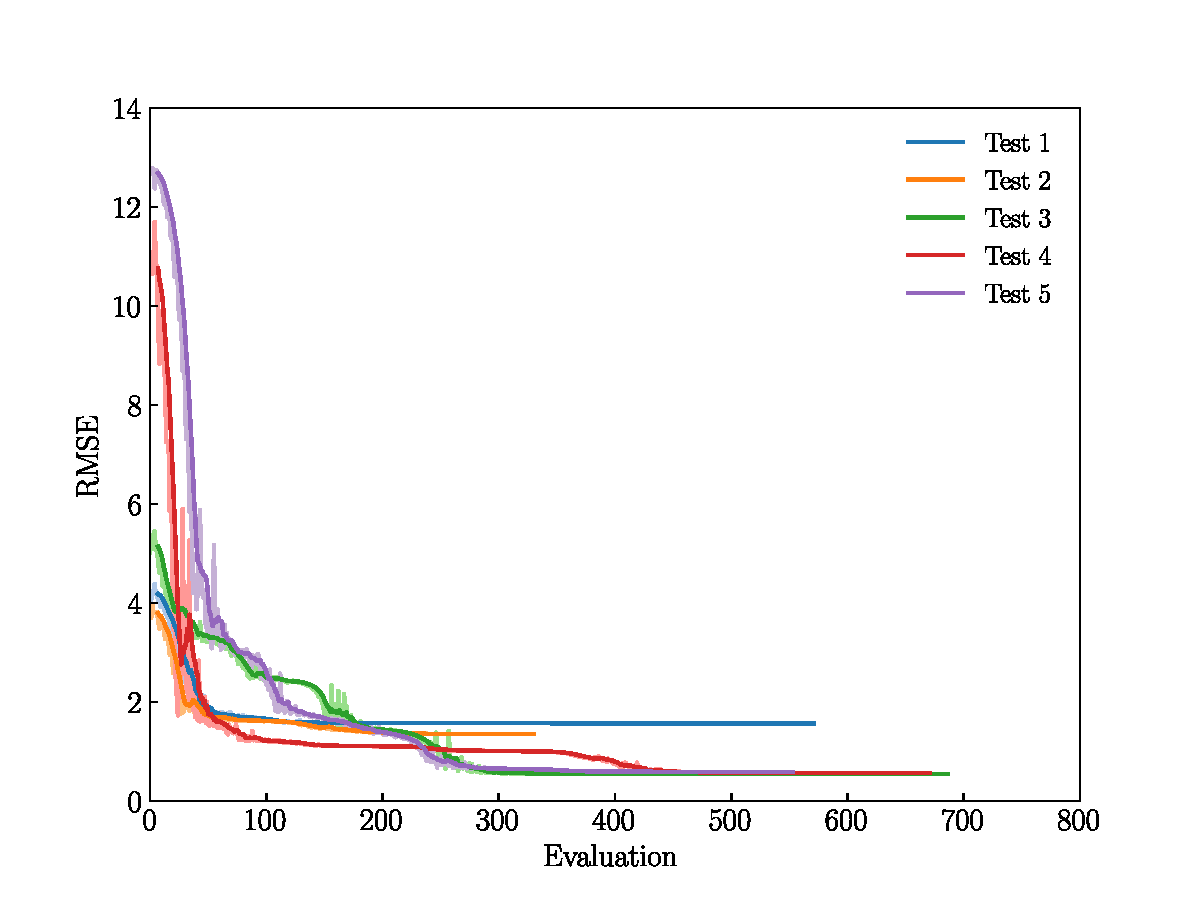
\includegraphics[width = 0.7\textwidth]{verify_rsme.pdf}
		\caption{rmse for multiple tests}
		\label{fig:rmse progress}
	\end{figure}

    
    \section{Validation}\label{sec: validation}
    To improve our algorithm we reduced the number of optimization parameters by fixing the elastic material parameters. The results of this implementation for three different data sets will be discussed in this section.

    \begin{figure}[H]
		\centering
        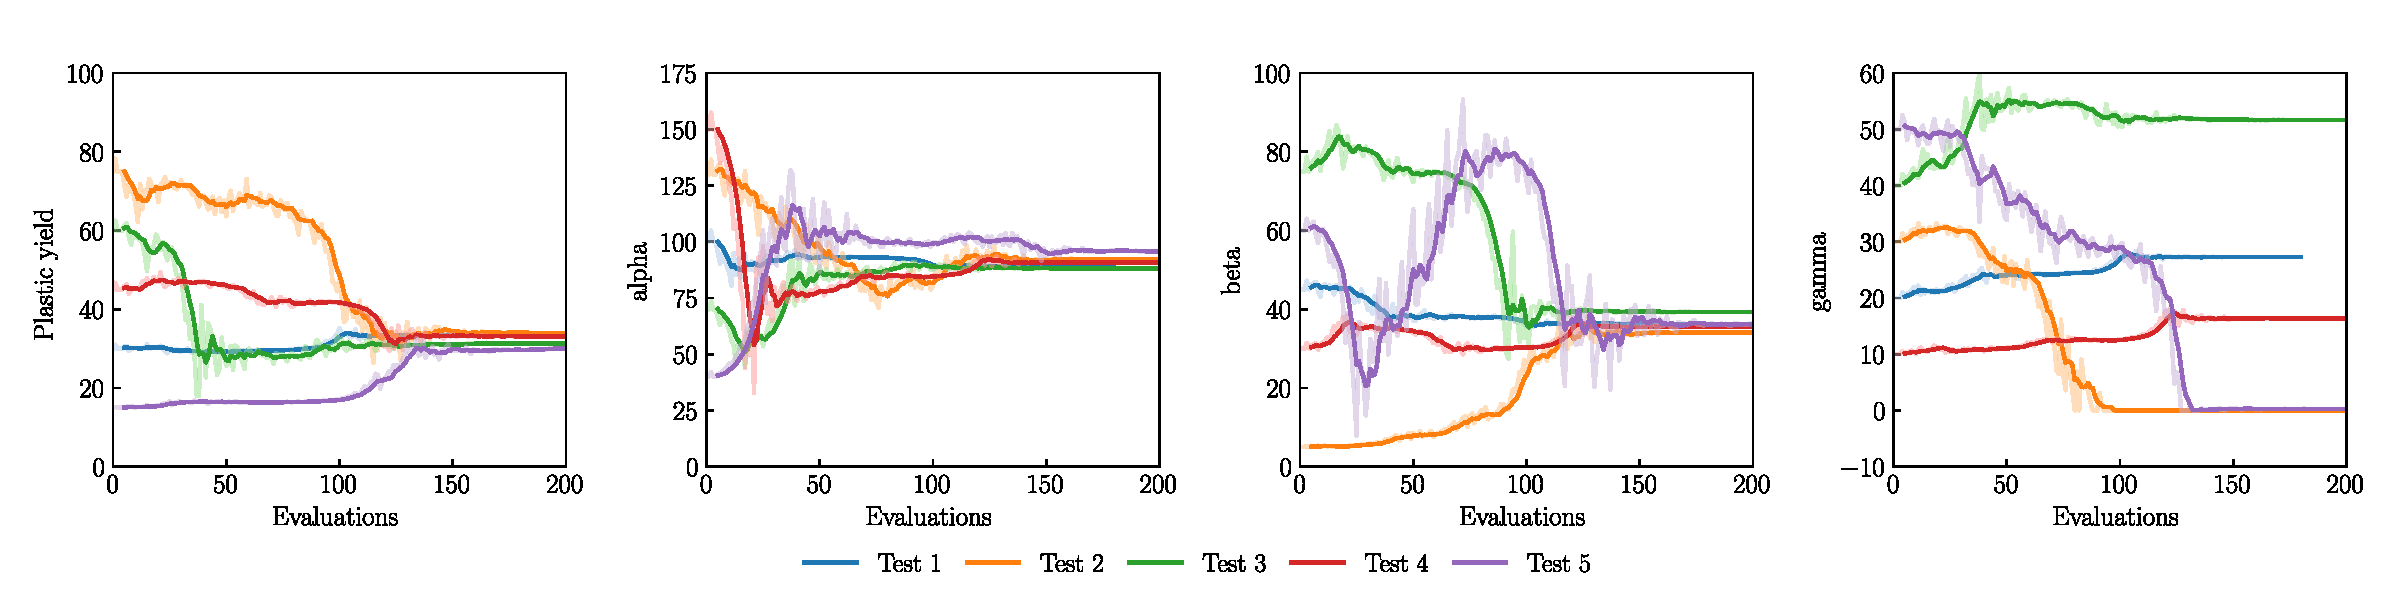
\includegraphics[width=0.47\textwidth]{valid6to3_material_params.pdf}
		\caption{progress of material parameters for validation tests}
		\label{fig:validation material params 6to3}
	\end{figure}

    In the first step we used the same data set as in \autoref{verification} to test the modified algorithm. The optimized plastic material parameters are shown in \autoref{fig:validation material params 6to3}.  In all tests, the values of the plastic yield, alpha and beta demonstrate a converging trend towards a singular solution. The only exception to this is gamma whose converged values vary for each individual test. As was outlined in the preceding discussion, gamma exerts minimal influence on the trend of the hardening curve. Consequently, the focus shall be directed towards the plastic yield, alpha and beta, which indicate an improvement in their optimization behavior.
    The quality of this optimized parameters is ensured through the match of the stress-strain curves with the target data. As demonstrated in \autoref{fig:validationStressStrain6to3} the final stress-strain curves exhibit a strong correlation with the target data. The evolution of the RMSE XXX supports this results with small values for every test. A comparison of the results of the present study with those of the verification study reveals an equivalent level of optimization quality. Additionally, the results of the material parameters indicate a positive impact of the algorithm modification, showing a unique solution for the important parameters. 
     
    
    \begin{figure}[H]
        \centering
        \begin{minipage}[t]{0.47\textwidth}
            \centering
            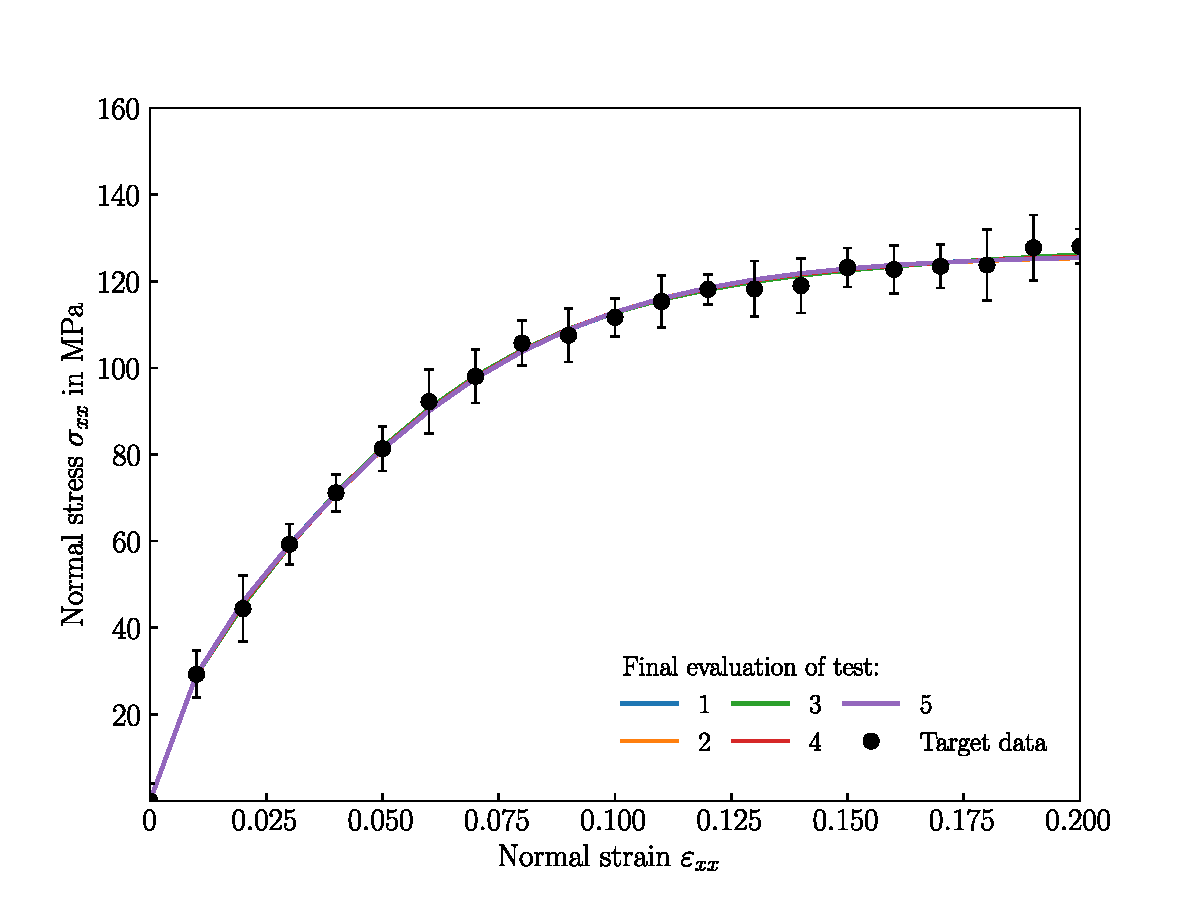
\includegraphics[width=\textwidth]{valid6to3_stress_strain_combined.pdf}
            \caption*{(a) Final stress-strain curves}
            \label{fig:validationStressStrain6to3}
        \end{minipage}
        \hfill
        \begin{minipage}[t]{0.47\textwidth}
            \centering
            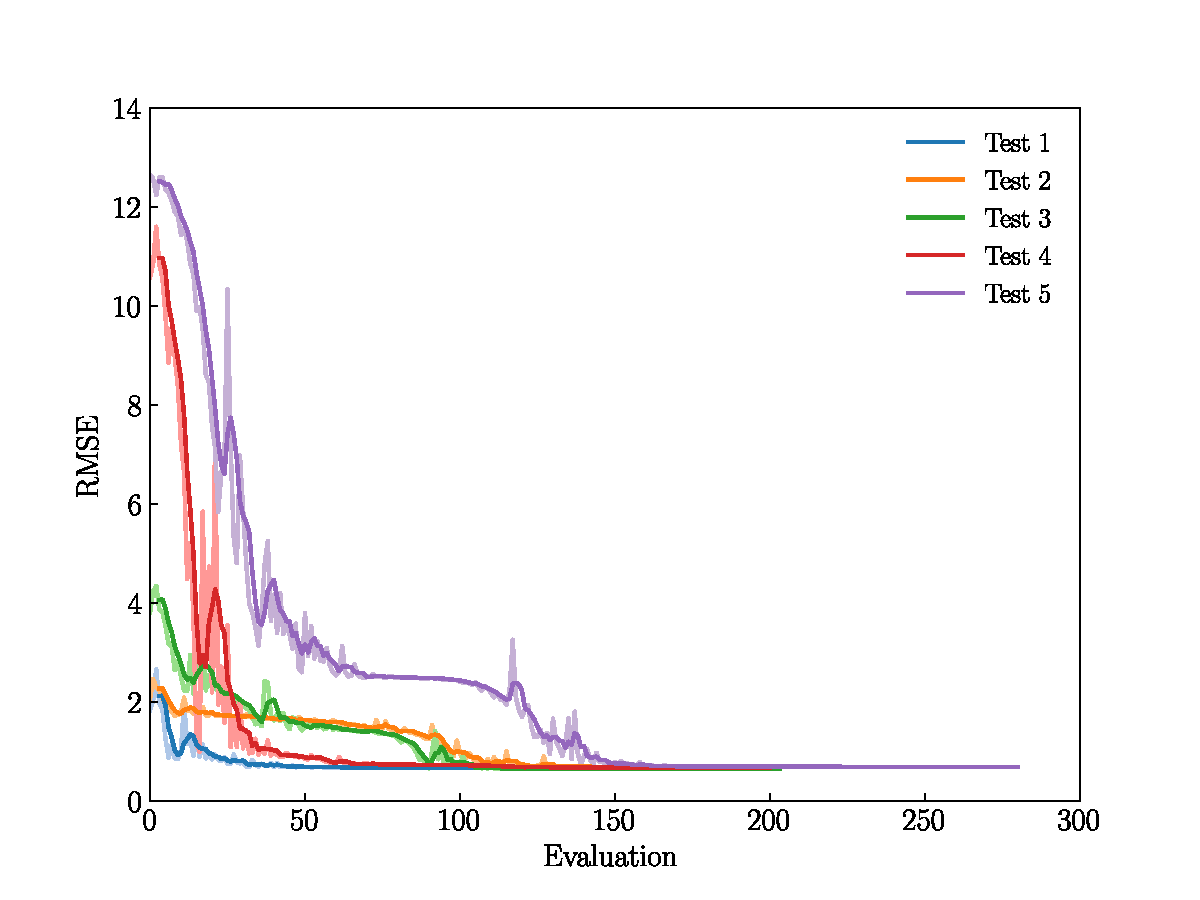
\includegraphics[width=\textwidth]{valid6to3_rsme.pdf}
            \caption*{(b) RMSE evolution}
            \label{subfigure:validation-rmse-6to3}
        \end{minipage}
        \caption{Results of validation tests with 6to3 dataset}
        \label{fig:validation results 6to3}
    \end{figure}
    


    To verify our algorithm independent of the used target data set, we made the same tests with two additional data sets. In the following we present the results of studies for mixing ratio 4:3 and 8:3. 

    \begin{figure}[H]
        \centering
        \subfigure[evolution of material 4:3]{
            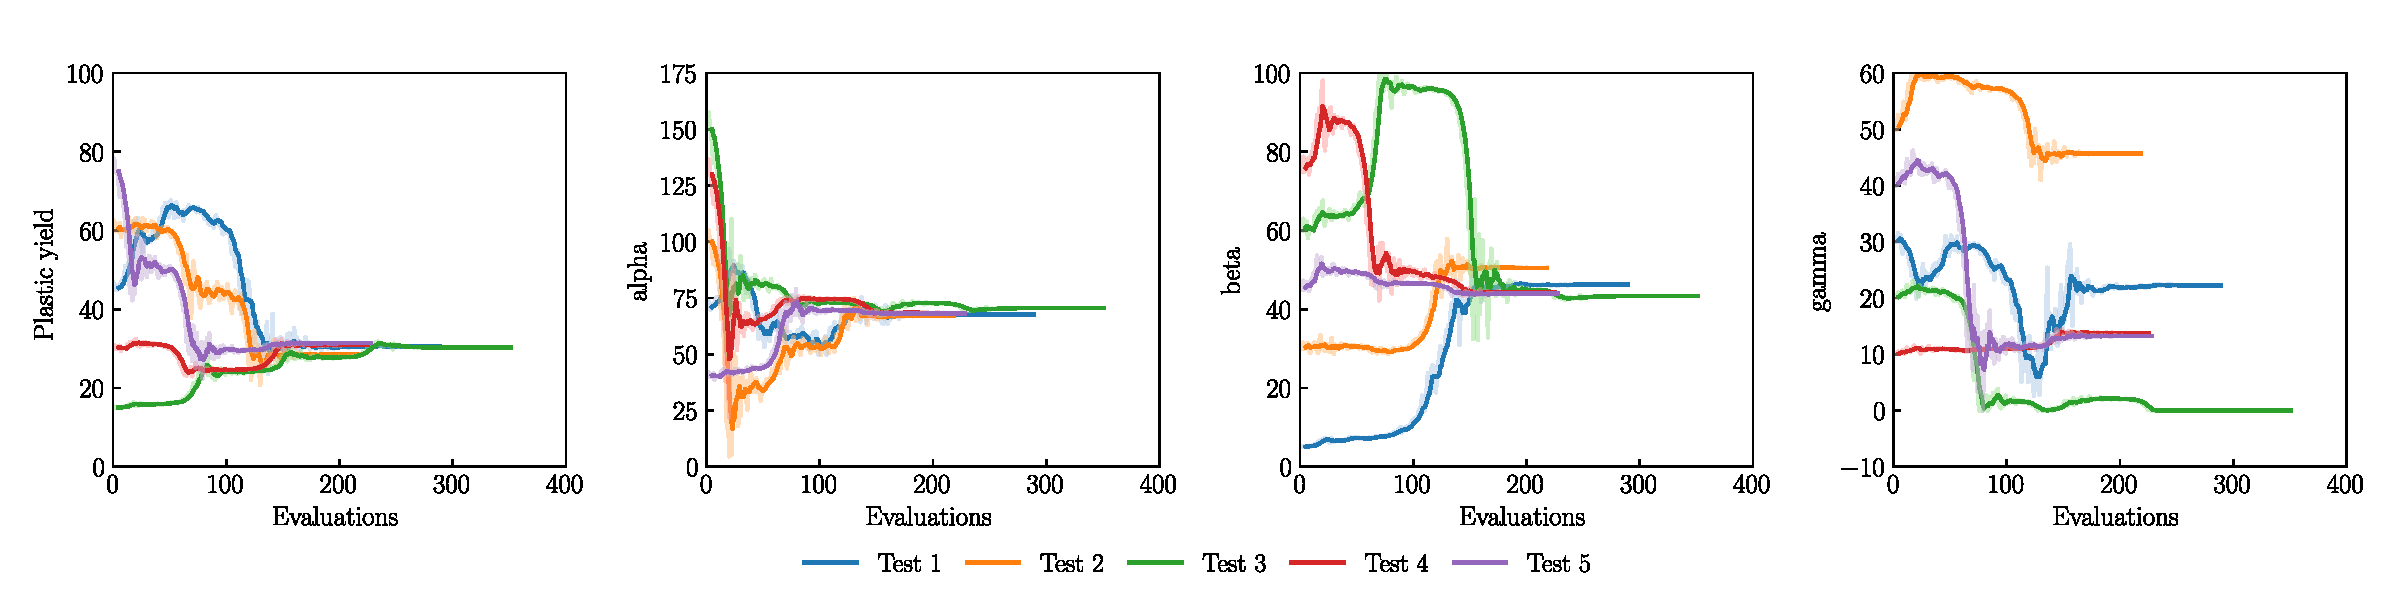
\includegraphics[width=1.0\textwidth]{valid4to3_material_params.pdf}
    		\label{fig:material params 4to3}
        }
        \subfigure[evolution of 8:4]{
            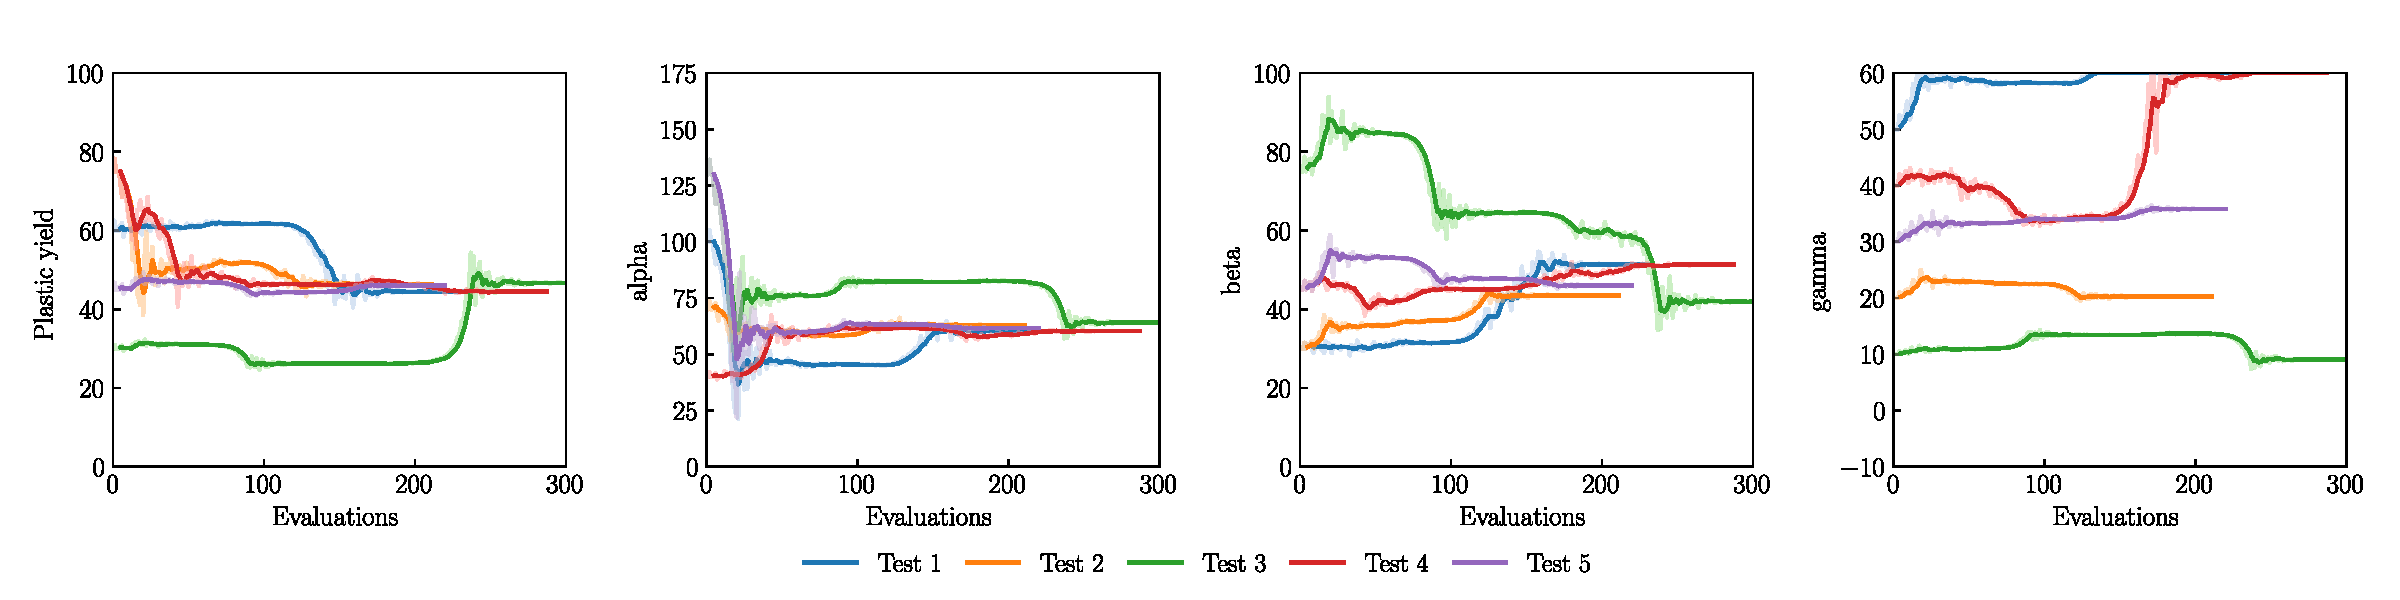
\includegraphics[width=1.0\textwidth]{valid8to3_material_paramspdf.pdf}
            \label{fig:material params 8to3}
        }
        \caption{Evolution of material parameters for a) mixing ratio 4:3 and b) mixing ratio 8:3}
        \label{fig:validation material params}
    \end{figure}

    The evolution of the plastic material parameters for the mixing ratios 4:3 and 8:3 in plotted in \autoref{fig:validation material params}. We can observe a similar convergence behaviour as in the validation study with mixing ratio 6:3. Only test case 3 for mixing ratio 8:3 shows a deviation provided that all values converge quite late. Since we chose the initial values randomly this might occur through an unfavourable combination of values. 
    In \autoref{fig:validation results} we represent the optimized stress-strain curves and the evolution of the RMSE. For all tests the stress-strain values correlate with the target data. The equivalent level of the RMSE for the converged solutions indicate a similar quality of the optimization result for all tests. These results indicate an improvement of the solution results through determining the elastic parameters.
     
    \begin{figure}[H]
        \centering
        \subfigure[stress-strain curves]{
            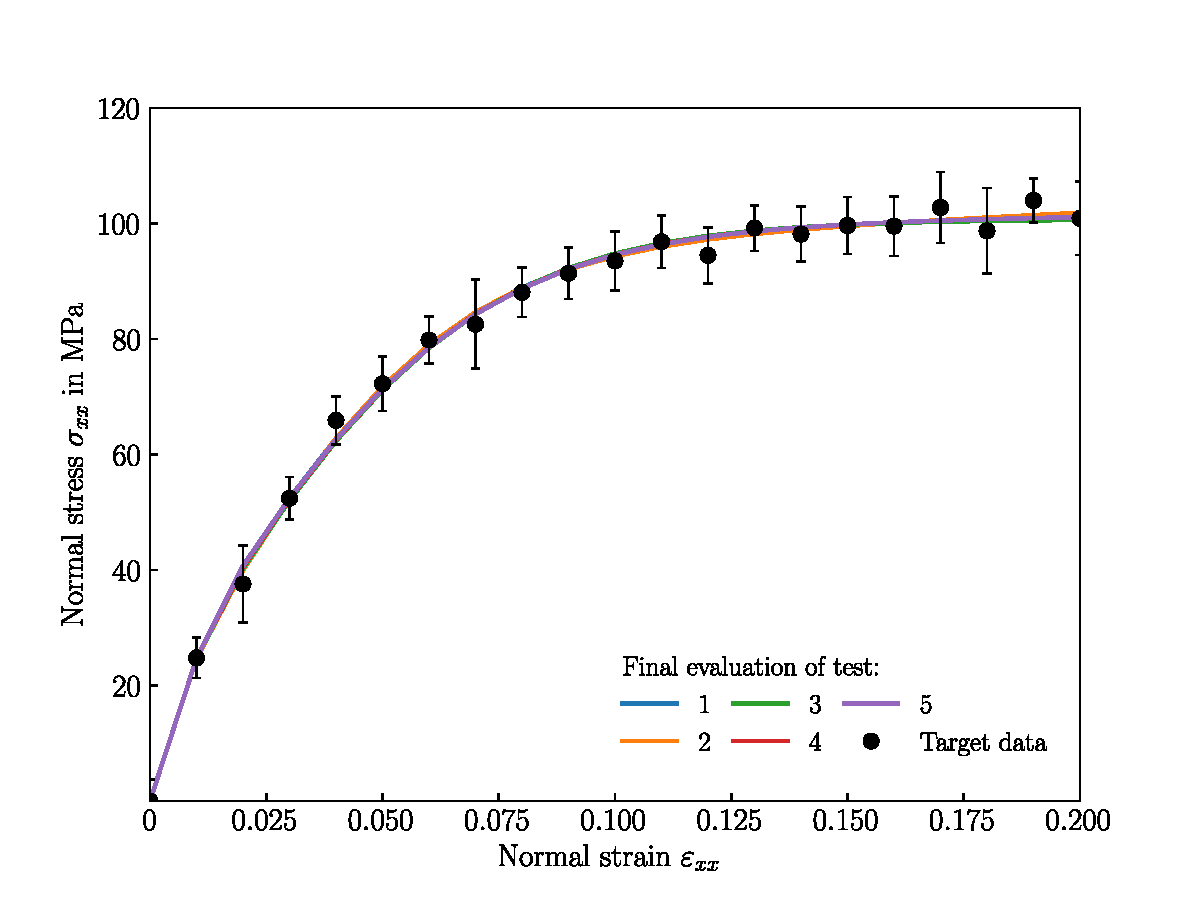
\includegraphics[width=0.47\textwidth]{valid4to3_stress_strain_combined.pdf}
    		\label{fig:validation stress-strain curves 4to3}
        }
        \subfigure[RMSE evolution]{
            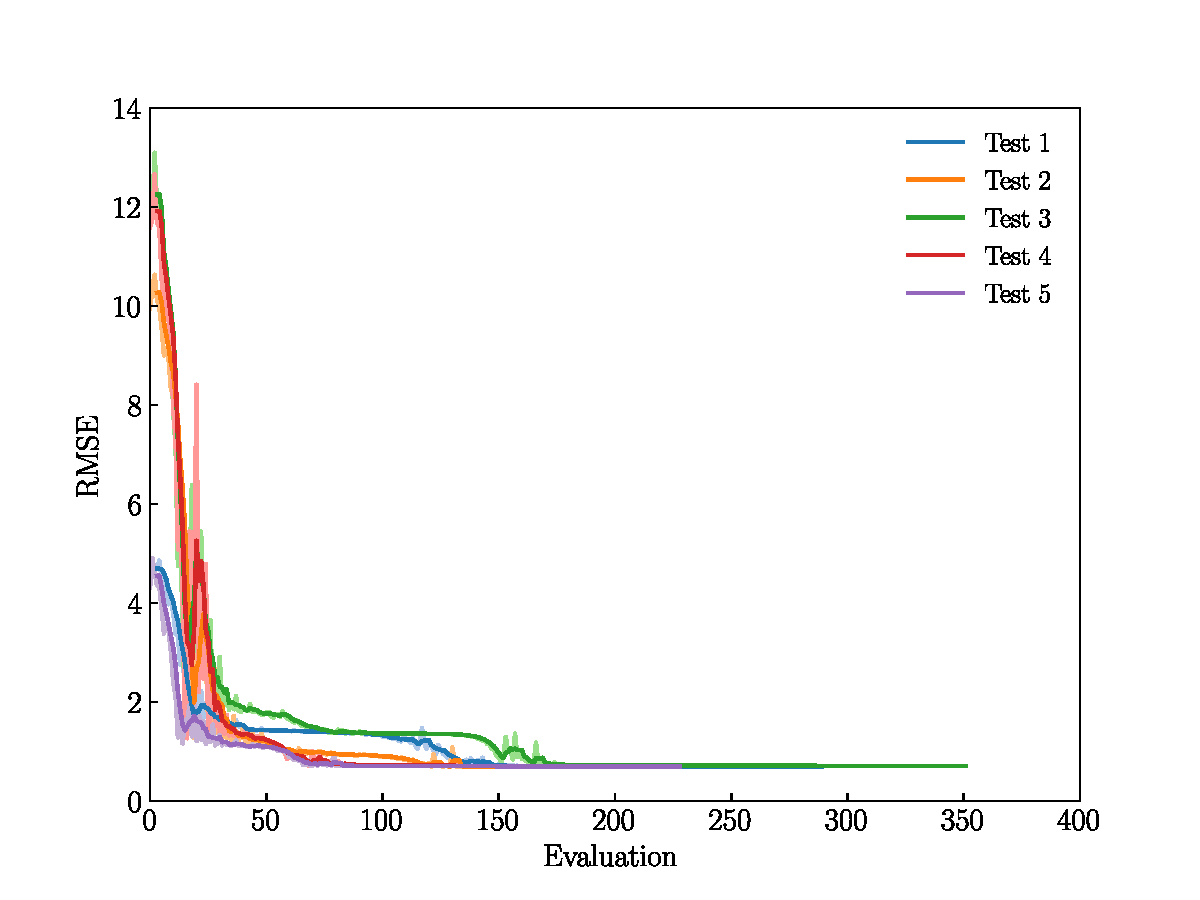
\includegraphics[width=0.47\textwidth]{valid4to3_rmse.pdf}
            \label{fig:validation rmse 4to3}
        }
        \subfigure[Final stress-strain curves]{
            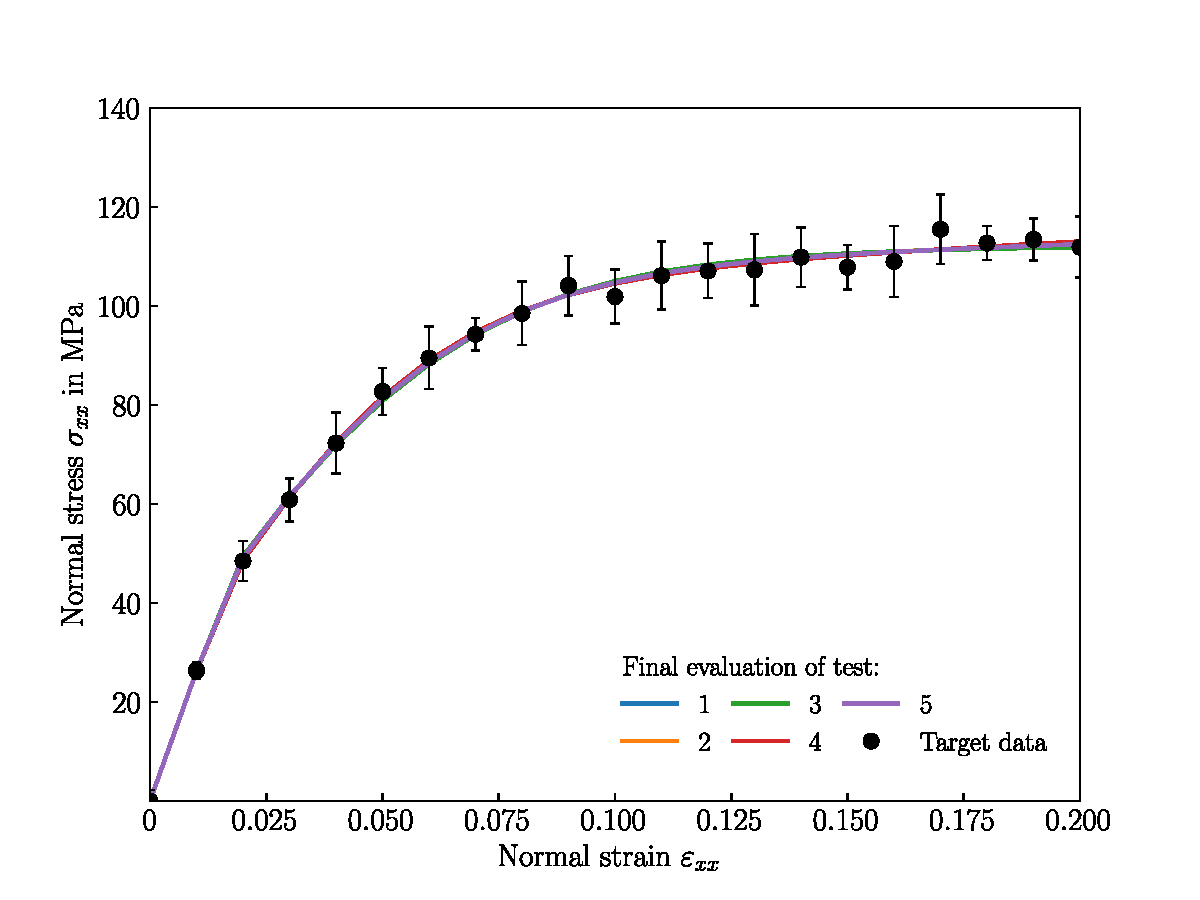
\includegraphics[width=0.47\textwidth]{valid8to3_stress_strain_combined.pdf}
    		\label{fig:validation stress-strain curves 8to3}
        }
        \subfigure[RMSE evolution]{
            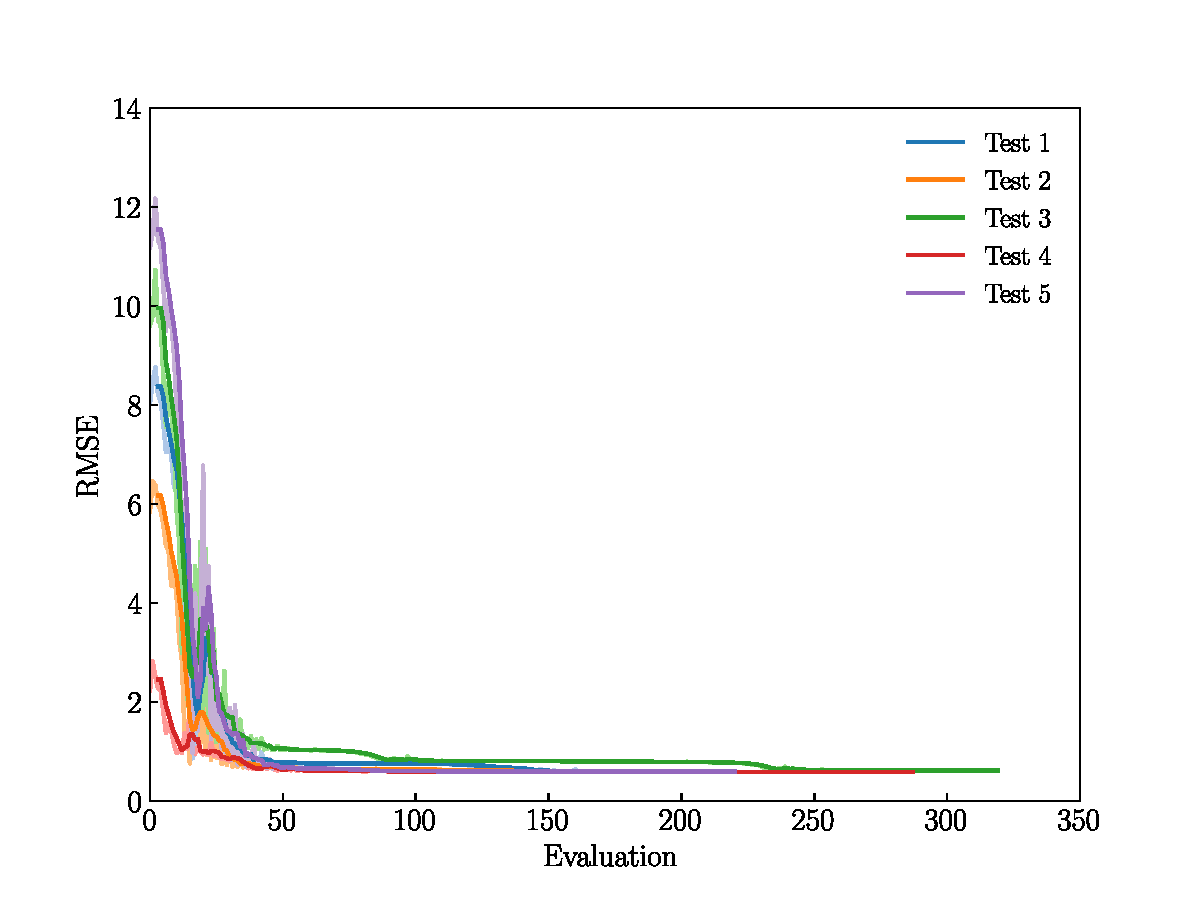
\includegraphics[width=0.47\textwidth]{valid8to3_rmse.pdf}
            \label{fig:validation rmse 8to3}
        }
        \caption{Results of validation tests with mixing ratios 4:3 and 8:3: a) final stress-strain curves for mixing ratio 4:3, b) RMSE for mixing ratio 8:3, c) final stress-strain curves for mixing ratio 4:3, d) RMSE for mixing ratio 8:3}
        \label{fig:validation results}
    \end{figure}

    Overall these results demonstrate the reliability of the optimization algorithm for the load case of a single tensile strain in one direction with fixed elastic parameters. The specification of the elastic parameter values improves the optimization performance in a way that for the plastic yield, alpha and beta independent of the initial values a singular solution can be found. However, the manual specification of Youngs modulus and Poisson ratio is only possible for target data sets with exactly one data point in the elastic domain of the material. For data sets with multiple points in the elastic domain a manual specification becomes complicated quite fast. Additional, for materials with completely unknown material behaviour, the point of transition between elastic and plastic behaviour is still unknown. In order to process such data sets too, we need to integrate the elastic parameters in the optimization process. In doing so the singularity of the solution should be maintained. Therefore the algorithm needs additional information about the mechanical material behaviour. In the following step we tried to do so through the combination of two load cases. Additional to the already tested tensile strain we applied a shear strain. As described in section XX the shear modulus contains information about Youngs modulus and  Poisson ratio what might improve the performance of the optimizatoin process. The information contained within the shear modulus about Youngs modulus and Poisson ratio might enclose the necessary restrictions to reduce the solution variability. 
    
    Warum sinusförmige belastung? Jz schon mit zyklischen versuchen kommen?
    

    \section{shear and normal strain tests combined}
    \section{cyclic tests}







	
    \chapter{Conclusion}


XX LITERATURBEZUG

\paragraph{Summary}
In this thesis, an optimisation approach to find material parameters for epoxies modelled with \acrshort{md} simulations, was developed. The mechanical behaviour of the material should be represented as good as possible through a constitutive model with corresponding material parameters. As constitutive model we use an elastoplastic model with a VOCE-hardening curve to describe the plastification. This model is defined with two elastic and four plastic material parameters. To monitor the quality of the material parameters, we perform simulations with the \acrshort{fe} software \name{Abaqus}. We implemented the whole optimisation procedure in a single \name{Python} script, since \name{Abaqus} has an \acrlong{api} which enables the control via \name{Python} commands. \\
Before we start the optimisation procedure, a model with specific properties is created in the preprocessing. The optimisation is started with an initial guess for the material parameters. With these parameters we perform the \acrshort{fe} simulation, and extract the resulting load reactions.
We compare the load reactions with the ones from the \acrshort{md} simulations, which we use as reference data.
The deviations are summarised in a single \acrshort{rmse} value.
This value is reduced through the numerical Nelder-Mead algorithm, which is able to optimise a scalar function in a multidimensional space. 
The algorithm adapts the material parameters and a new evaluation starts. 
To verify the algorithm, we used reference data from \acrshort{md} simulations performed by \citet{ries_deciphering_nodate} for materials with mixing ratio 6:3, where a linear tensile strain up to a maximum strain of 20\% was applied.
We performed tests with the same loading conditions for materials with mixing ratio 4:3, 6:3 and 8:3 to validate the performance of the approach. 
For material with mixing ratio 6:3, we applied sinusoidal strain up to a maximum amplitude of 15\%. 
We performed optimisation tests with these load parameters as tensile loading, shear loading, and finally their combination. 
In the final tests, we applied 1.5 loading cycles of sinusoidal tensile strains with 1, 5 and 8\% amplitude.

\paragraph{Conclusion}
The developed optimisation approach is able to minimise the error between the reference data and the \acrlong{olr} through adaption of the material parameters. The verification study showed, that the optimisation procedure achieves a perfect match of the load reactions for pure tensile loading through a linear strain application. However, the identified material parameters strongly deviate within the test series. We attribute this behaviour to the relatively high number of optimisation variables. Therefore, we predefined the elastic parameters $E$ and $\nu$, and optimised the plastic parameters. With this adaption we can affirm the second research question. In the validation study, the code reliably found similar material parameters independent of the initial value combination. In addition, the \acrlong{omp} agree with the reference values found by \citet{ries_deciphering_nodate}.
The studies using sinusoidal load application provide information about the algorithm performance in different load cases. The pure tensile loading led to results of similar quality as the validation study, whereas in the shear load case problems about the optimisation of the plastic yield occurred.
Possible reasons for this behaviour were discussed in \autoref{subsec:CombiDiscussion}. In the reference data for the cyclic tests, the material properties change during the loading process, which might be explained through arising material damage. Since we disregarded damage models in our \name{Abaqus} simulation, the \acrlong{olr} show high variations from the reference data. The tests demonstrated, that from the tested loading procedures, optimisation of tensile loadings gives reliable results. For the other tested configurations, the results of the material parameters are still arbitrary.


\paragraph{Outlook}
The processing of shear load cases should be part of future investigations. Here, the focus should be taken on the transition from elastic to plastic material behaviour.
The tests performed in this work demonstrate open issues with the definition of the yield stress, which represents the starting point of the plastic regime. 
For an adequate representation of cyclic loading, a damage model should be included in the \name{Abaqus} model.
Because of unusual material behaviour, a subroutine would be necessary. 
Furthermore, the properties of the numerical optimisation algorithm could be part of future investigations.
Here, the initial value combinations were picked arbitrary.
Since this may lead to getting stuck in local minima, the impact of the initial value combination on the optimisation process should be studied. In addition, the choice of the numerical algorithm could be reflected.
The sensitivity of the algorithm to the initial values could be reduced by choosing alternatives. 

% Summary: 
% - script for optimisation
% - md simulations cannot define matrial params

% - fem sim necessary to do thi (continuum based approach)
% - try to fit mechanical behaviour from md sim with const model and corresponding mat params
% - do this via optimisation
% - minimise the diff of the mechanical resp of md and fem through optimisation of mat params
% - via python script in abaqus python interface
% - use nelder mead alg and rmse to reduce diff

% Conclusion:
% 1. yes: verification showed: script minimises rmse, the load reactions match perfectly
% but2: no unique solution for the mat params --> fix elastic params, since only one point in the elastic regime

% 2. yes in validation study: if elast params are fixed, the other params can be determined independent of the initial val combi, except gamma but gamma has only a small effect on the trend of the hardening curve --> not important 

% 3.: verification and validaiton: for linear tensile load works fine 
% tensile: tensile as sin function works too
% shear: yield stress runs into limit in all tests --> difiiculties in finding limit between el and plastic domain
% tensile and shear combined: problems of shear are transferred, and elastic params are not similar --> not possible to match obth curves at a time --> error much higher than before, plot stress strain tens 
% cyclic: works just until unloading stars, because of material damage, cannot represent mat damage, because elastic behaviour is influenced too --> have to write own usersubroutine 

% conclusion: 
% userfriednly: only input file must be adapted 
% everything in one script, automatic data storage
% dynamic adaption for various loading combinations (mult load params, load cases, initial value combinations)
% optimisation script generally works for tensile load application for different load parameters
% for shear load problems at differnetiation between el and plast regime 
% for cyclic damage inclusion
% md data maybe not perfectly suitable

% outlook: 
% - for shear load improvement of differnetiation between el and plast regime 
% - for cyclic damage inclusion
% - more equivalent distribution of reference data points in the domain --> more elastic points
% - ensrue reliability of relaxation procedure for shear loading




    
    
	

	
	
	
	\clearpage
	\newpage
	 \pagenumbering{roman}
	%----------------------------------------------
	% Bibliograhy
	%----------------------------------------------
	%\nocite{*} %print every bibtex key
	
	\pagestyle{fancy}
	\fancyhead{}
	\fancyfoot{}
	% one sided 
	\fancyhead[R]{\rightmark}
	\renewcommand{\headrulewidth}{0.4pt}
	\fancyfoot[R]{\thepage}
	\renewcommand{\chaptermark}[1]{\markboth{\thechapter\ #1}{}}
	\renewcommand{\sectionmark}[1]{\markright{\thesection\ #1}}
	
	\printbibliography[heading=bibintoc, title={Bibliography}]
	
	\newpage
	
	%\addtocontents{toc}{\protect\setcounter{tocdepth}{0}}
	\begin{appendices}
    \chapter{Appendix}
    \section{Results}


    \begin{figure}[H]
    \centering
    \begin{subfigure}[t]{1.0\textwidth}
        \centering
        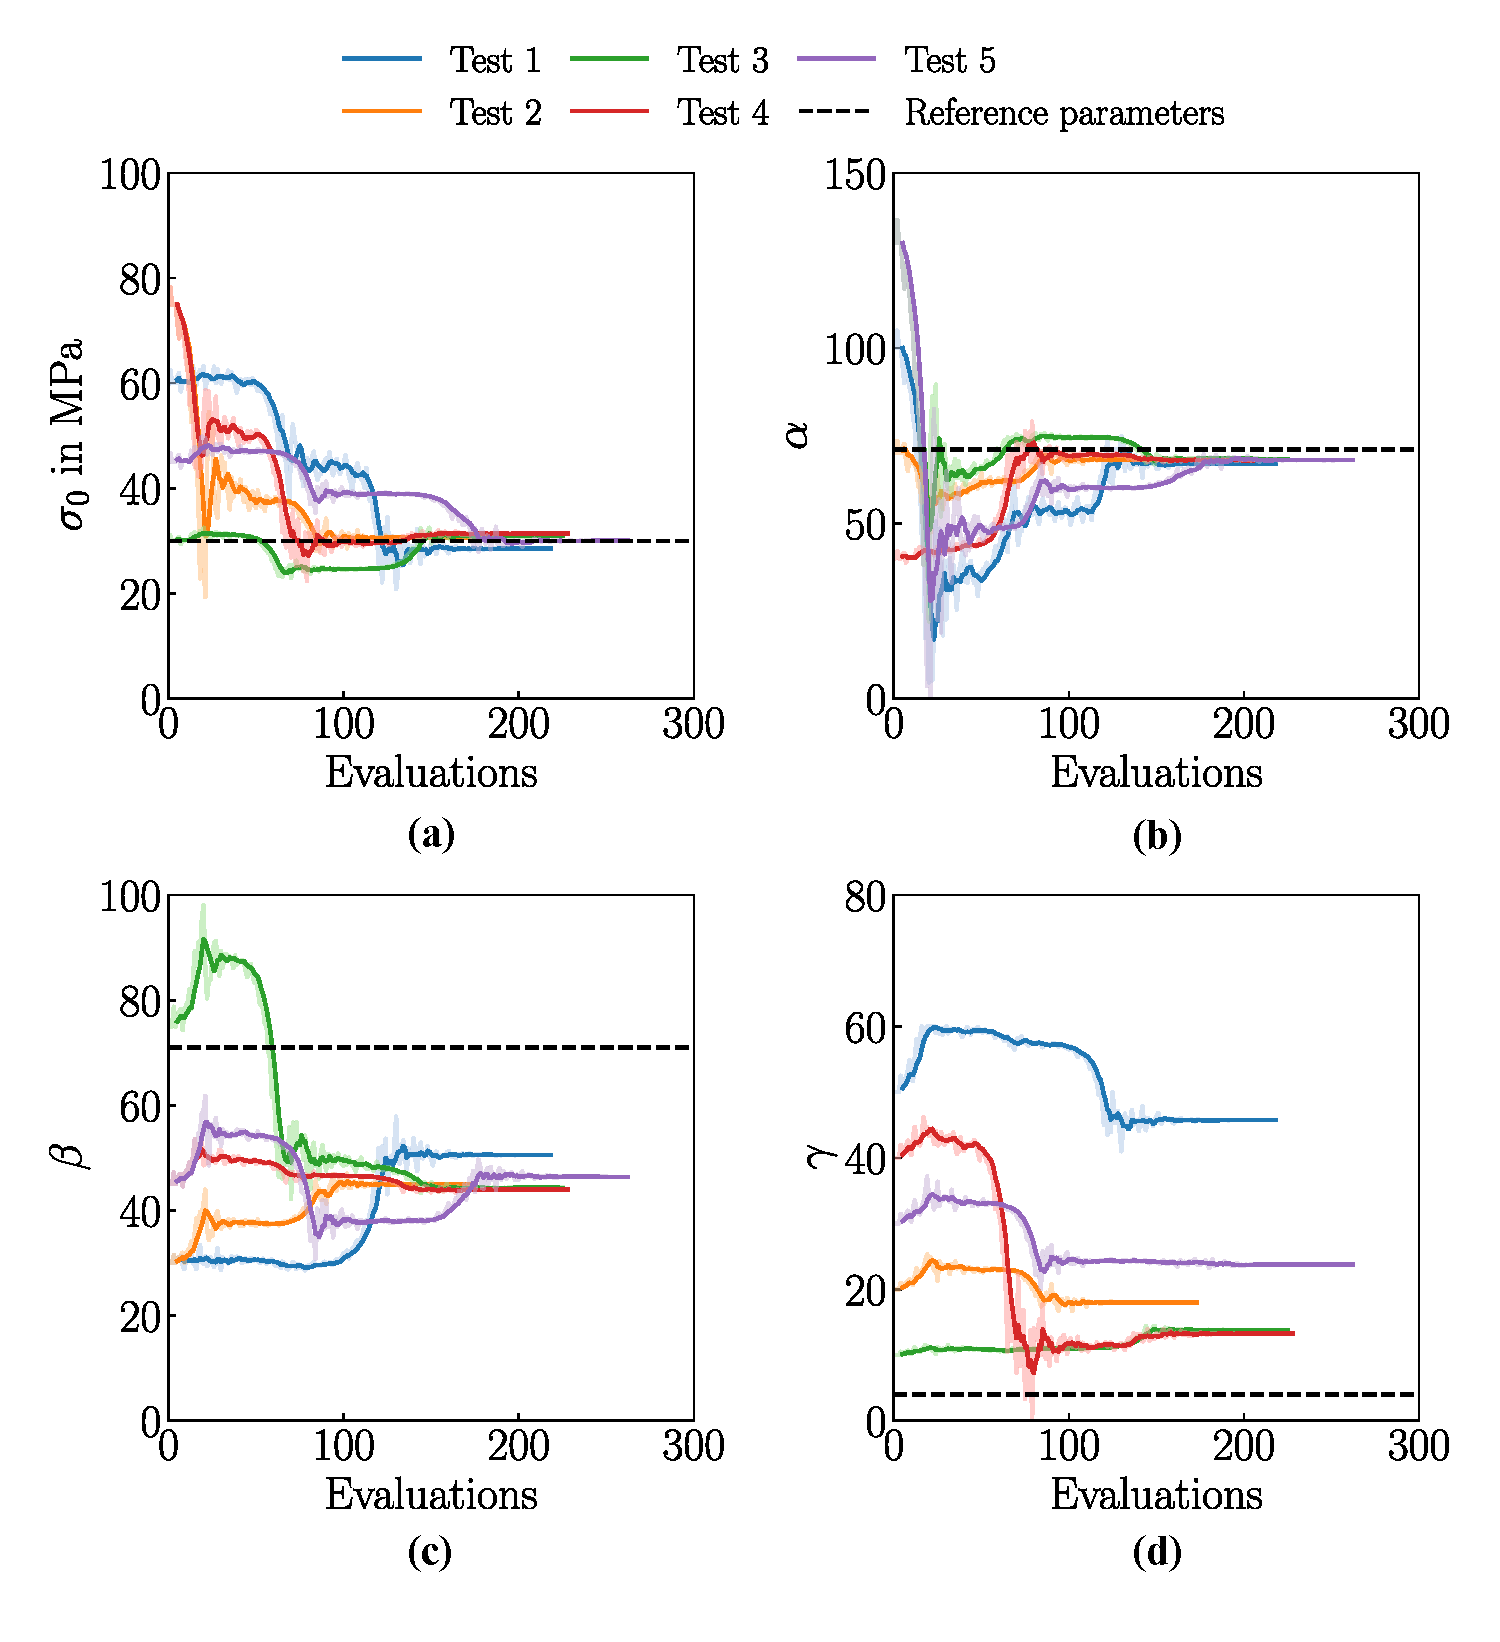
\includegraphics[width=0.66\textwidth]{Vald_4To3_fixEP1_material_params.pdf}
        \caption{Evolution of material 4:3}
        \label{fig:material_params_4to3}
    \end{subfigure}
    \begin{subfigure}[t]{1.0\textwidth}
        \centering
        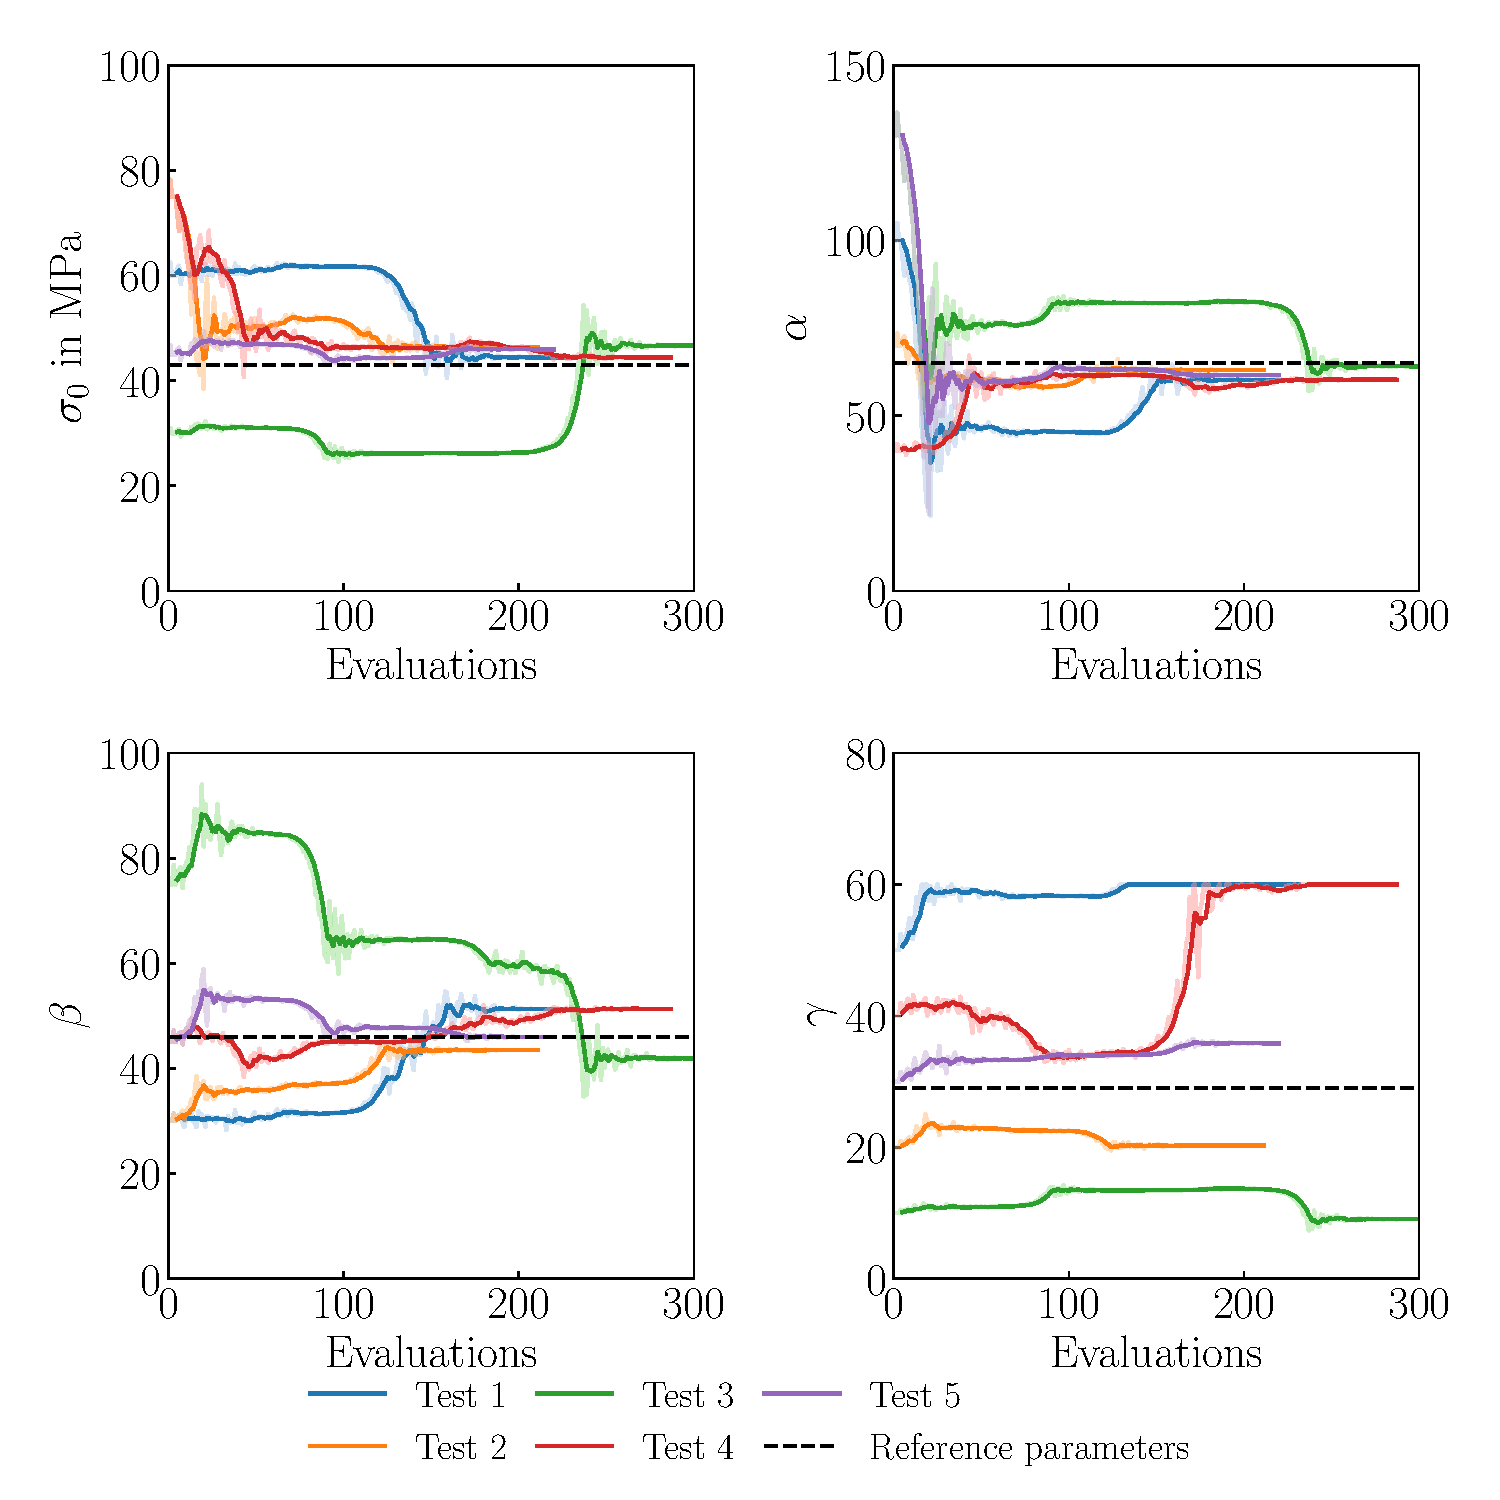
\includegraphics[width=0.66\textwidth]{Vald_8To3_fixEP1_material_params.pdf}
        \caption{Evolution of 8:3}
        \label{fig:material_params_8to3}
    \end{subfigure}
    \caption{Evolution of material parameters for (a) mixing ratio 4:3 and (b) mixing ratio 8:3.}
    \label{fig:validation_material_params}
    \end{figure}
    \chapter{Appendix}
\end{appendices}
	
	\end{document}
